\documentclass{article}

\usepackage[utf8]{inputenc}
\usepackage{amsmath, mathrsfs}
\usepackage{amssymb}
\usepackage{enumerate}
\usepackage{tikz}
\usepackage{tensor}
\usepackage[italicdiff]{physics}
\usepackage{amsfonts}
\usepackage{graphicx}
\usepackage{tabularx}
\usepackage[left = 3.5cm, right = 3.5cm, top=3cm, bottom=3cm]{geometry}
\usepackage{hyperref, color}
\hypersetup{
    colorlinks=False,
    linktoc=all,     %set to all if you want both sections and subsections linked
}
\usepackage{mathtools}
\newcommand{\defeq}{\vcentcolon=}
\newcommand{\overbar}[1]{\mkern 1.5mu\overline{\mkern-1.5mu#1\mkern-1.5mu}\mkern 1.5mu}
\newcommand{\infint}{\int_{-\infty}^{\infty}}
\numberwithin{equation}{section}

\usepackage{amsthm}

\theoremstyle{definition}
\newtheorem*{law}{Law}
\newtheorem*{definition}{Definition}
\newtheorem*{proposition}{Proposition}
\newtheorem*{theorem}{Theorem}
\newtheorem*{example}{Example}
\newtheorem*{corollary}{Corollary}
\newtheorem*{lemma}{Lemma}
\newtheorem*{note}{Note}

\usepackage{fancyhdr}
\pagestyle{fancy}


\usetikzlibrary{arrows.meta}
\usetikzlibrary{decorations.markings}
\usetikzlibrary{decorations.pathmorphing}
\usetikzlibrary{positioning}
\usetikzlibrary{fadings}
\usetikzlibrary{intersections}
\usetikzlibrary{cd}
\usetikzlibrary{calc}

\tikzset{>={Latex[length=2mm]}}

\tikzset{
    set arrow inside/.code={\pgfqkeys{/tikz/arrow inside}{#1}},
    set arrow inside={end/.initial=>, opt/.initial=},
    /pgf/decoration/Mark/.style={
        mark/.expanded=at position #1 with
        {
            \noexpand\arrow[\pgfkeysvalueof{/tikz/arrow inside/opt}]{\pgfkeysvalueof{/tikz/arrow inside/end}}
        }
    },
    arrow inside/.style 2 args={
        set arrow inside={#1},
        postaction={
            decorate,decoration={
                markings,Mark/.list={#2}
            }
        }
    },
}
\def\centerarc[#1](#2)(#3:#4:#5)% Syntax: [draw options] (center) (initial angle:final angle:radius)
    { \draw[#1] ($(#2)+({#5*cos(#3)},{#5*sin(#3)})$) arc (#3:#4:#5); }
\newcommand{\R}{\mathbb{R}}
\newcommand{\C}{\mathbb{C}}
\newcommand{\Z}{\mathbb{Z}}
\newcommand{\N}{\mathbb{N}}
%\renewcommand{\dv}[3][]{\frac{d^{#1} #2}{d#3^{#1}}}
\newcommand{\dotp}[2]{#1 \cdot #2}
\renewcommand{\cp}[2]{#1 \times #2}
\renewcommand{\grad}[1]{\vec{\nabla} #1}
\renewcommand{\div}[1]{\vec{\nabla} \cdot #1}
\renewcommand{\curl}[1]{\vec{\nabla} \times #1}
\renewcommand{\infint}{\int_{-\infty}^{\infty}}
\newcommand{\oinfint}{\int_0^\infty}
\renewcommand{\implies}{\quad \Rightarrow \quad}
\newcommand{\qqr}[1]{\quad \text{#1}}
\newcommand{\equivalent}{\quad \Leftrightarrow \quad}

% tikz commands
\usetikzlibrary{shapes.misc}
\usetikzlibrary{math}
\tikzset{cross/.style={cross out, draw=black, fill=none,minimum size=2*(#1-\pgflinewidth), inner sep=0pt, outer sep=0pt}, cross/.default={2pt}}
\def\vectorin[#1](#2)% Syntax: [size in pt] (coordinate)
{ \filldraw[fill=white] (#2) circle (sqrt 2*#1) node[cross= #1] {}; }
%{ \draw (#2) circle (sqrt 2*#1) node[cross= #1, fill=white] {}; }
\def\vectorout[#1](#2)
{ \filldraw[fill=white] (#2) circle(5*#1 pt) node[circle,fill=black,inner sep=#1pt] {};}

\usetikzlibrary{decorations.pathmorphing,patterns}

\begin{document}
	\begin{titlepage}
		\vspace*{\fill}
		\begin{center}
			{\Huge{\textbf{Classical Mechanics}}}\\[2cm]
			{\large{Emre Özer}\\[0.1cm]}
			February 2020 \\
			\vspace{4mm}
			Notes based on Claudia de Rham's lectures at Imperial College and David Tong's notes on Classical Dynamics.
		\end{center}
		\vspace*{\fill}
	\end{titlepage}
	
	\tableofcontents
	\newpage

\section{Rigid Body Rotation}
\textit{(Summation convention sometimes used in this chapter, should be clear from context.)}
\subsection{Basics of rigid bodies}
A body is a collection of particles. We consider a set of $N$ particles with positions $\vec{r}_{a}(t)$ and masses $m_{a}$, where $a = 1, \dots, N$. Each particle obeys the equation of motion
\begin{equation}
	m_{a}\ddot{\vec{r}}_a = \sum_{b \neq a} \vec{F}_{ab} + \vec{F}_a^{\mathrm{ext}},
\end{equation}
where $\vec{F}_{ab}$ is the force on particle $a$ due to $b$ and $ \vec{F}_{a}^{\text{ext}} $ is the sum of all external forces on $ a $. It is mathematically convenient to define $\vec{F}_{aa} \equiv 0$ and to take the sum over all $b$ instead of over $b \neq a$.
\par
The total mass $M$ of the body is
\begin{equation}
    M = \sum_a m_a.
\end{equation}
The centre of mass $\vec{R}$ is defined as
\begin{equation}
    \vec{R} = \frac{1}{M} \sum_a m_a \vec{r}_a \implies \dot{\vec{R}} = \frac{1}{M} \sum_a m_a \dot{\vec{r}}_a,
\end{equation}
which is just a weighted average with weights of $\flatfrac{m_{a}}{M}$. In the continuum limit, we have
\begin{equation}
    m_a \to \rho(\vec{r}) \implies M = \int_V \rho(\vec{r}) \dd[3]{r}, \qq{and} \vec{R} = \frac{1}{M} \int_V \rho(\vec{r}) \vec{r} \dd[3]{r}.
\end{equation}
Similarly, the total momentum $\vec{P}$ of the body is
\begin{equation}
    \vec{P} = \sum_a \vec{p}_a = \sum_a m_a \dot{\vec{r}}_a = M \dot{\vec{R}}.
\end{equation}
It then follows that
\begin{equation}
    \dot{\vec{P}} = \sum_a m_a \ddot{\vec{r}}_a = \sum_a \qty(\sum_b \vec{F}_{ab} + \vec{F}^{\text{ext}}_a) = \sum_{ab} \vec{F}_{ab} + \sum_a \vec{F}^{\text{ext}}_{a}.
\end{equation}
By Newton's third law, we have 
\begin{equation}
    \vec{F}_{ab} = - \vec{F}_{ba} \implies \sum_{ab} \vec{F}_{ab} \equiv 0.
\end{equation}
Hence, we have
\begin{equation}
    \dot{\vec{P}} = M \ddot{\vec{R}} = \sum_a \vec{F}^{\text{ext}}_{a}.
\end{equation}
So, total momentum of the body is conserved if no external forces act on the body with internal forces having no effect.
\par
The total angular momentum $\vec{L}$ is
\begin{equation}
    \vec{L} = \sum_a \vec{\ell}_a = \sum_a \vec{r}_a \times \vec{p}_a = \sum_a m_a \vec{r}_a \times \dot{\vec{r}}_a.
\end{equation}
The rate of change of total angular momentum is then
\begin{align}
    \begin{split}
        \dot{\vec{L}} = \sum_a m_a \dv{}{t} \qty(\vec{r}_a \times \dot{\vec{r}}_a) &= \sum_a m_a \qty(\dot{\vec{r}}_a \times \dot{\vec{r}}_a + \vec{r}_a \times \ddot{\vec{r}}_a) \\
        &= \sum_a m_a  \vec{r}_a \times \ddot{\vec{r}}_a \\
        &= \sum_a  \vec{r}_a \times \qty(\sum_b \vec{F}_{ab} + \vec{F}_a^{\text{ext}}) \\
        &= \sum_{ab} \vec{r}_a \times \vec{F}_{ab} + \sum_a \vec{r}_a \times \vec{F}_a^{\text{ext}}.
    \end{split}
\end{align}
Let's inspect the first term. It follows from Newton's third law that
\[
    \sum_{ab} \vec{r}_a \times \vec{F}_{ab} = - \sum_{ab} \vec{r}_a \times \vec{F}_{ba}.
\]
Since the indices $a$ and $b$ are dummy indices, we can relabel $a \leftrightarrow b$ to obtain
\begin{equation}
     \sum_{ab} \vec{r}_a \times \vec{F}_{ab} = \sum_{ab} -\vec{r}_b \times \vec{F}_{ab} \implies \sum_{ab} \vec{r}_a \times \vec{F}_{ab} = \frac{1}{2} \sum_{ab} (\vec{r}_a - \vec{r}_b) \times \vec{F}_{ab}.
\end{equation}
If the inter-particle forces are \textit{central}, the force $\vec{F}_{ab}$ points in the direction of the separation vector $\vec{r}_{ab} \equiv \vec{r}_a - \vec{r}_b$. Hence, the contribution above becomes identically zero and we get
\begin{equation}
    \dot{\vec{L}} = \sum_a \vec{r}_a \times \vec{F}_a^{\text{ext}} \equiv \vec{\tau},
\end{equation}
where $\vec{\tau}$ is the total torque on the body due to external forces. We again see that the inter-particle forces are \textit{averaged out} as far as the total angular momentum is concerned.
\par
Finally, we look at how the motion of the body decouples into centre of mass motion and relative motion about the centre of mass. We define the position relative to the centre of mass:
\begin{equation}
    \vec{r}^{\,*} = \vec{r} - \vec{R}.
\end{equation}
Then, we have
\begin{equation}
    \sum_a m_a \vec{r}^{\,*}_a = \sum_a m_a \qty(\vec{r}_a - \vec{R}) = M\vec{R} - M \vec{R} \equiv 0,
\end{equation}
as expected. The total linear momentum about the centre of mass is also identically zero,
\begin{equation}
    \vec{P}^{\,*} = \sum_a m_a \vec{r}^{\,*}_a = \sum_a m_a (\vec{r}_a - \vec{R}) = M\vec{R} - M\vec{R} \equiv 0 \implies \dot{\vec{P}}^{\,*} \equiv 0.
\end{equation}
The total angular momentum is expressed in terms of $\vec{r}^{\,*}_a$ as follows:
\begin{align}
    \begin{split}
        \vec{L} = \sum_a m_a \vec{r}_a \times \dot{\vec{r}}_a &= \sum_a m_a \qty(\vec{r}^{\,*}_a + \vec{R}) \times \qty(\dot{\vec{r}}^{\,*}_a + \dot{\vec{R}}) \\
        &= \sum_a m_a \qty[ \vec{r}^{\,*}_a \times \dot{\vec{r}}^{\,*}_a + \vec{r}^{\,*}_a \times \dot{R} + \vec{R} \times \dot{\vec{r}}^{\,*}_a + \vec{R} \times \dot{\vec{R}}] \\
        &= \sum_a m_a \vec{r}^{\,*}_a \times \dot{\vec{r}}^{\,*}_a + \qty(\sum_a m_a \vec{r}^{\,*}_a) \times \dot{R} + \vec{R} \times \qty(\sum_a m_a \dot{\vec{r}}^{\,*}_a) + M \vec{R} \times \dot{\vec{R}} \\
        &= \sum_a m_a \vec{r}^{\,*}_a \times \dot{\vec{r}}^{\,*}_a + \vec{R} \times \vec{P} \\
        &\equiv \vec{L}^{\,*} + \vec{R} \times \vec{P},
    \end{split}
\end{align}
where we defined the angular momentum about the central mass $\vec{L}^{\,*} = \sum_a m_a \vec{r}^{\,*}_a \times \dot{\vec{r}}^{\,*}_a$. The rate of change of $\vec{L}^{\,*}$ is given by
\begin{align}
    \begin{split}
        \dot{\vec{L}}^{\,*} = \sum_a m_a \vec{r}^{\,*}_a \times \ddot{\vec{r}}^{\,*}_a &= \sum_a m_a \qty(\vec{r}_a - \vec{R}) \times \qty(\ddot{\vec{r}}_a - \ddot{\vec{R}}) \\
        &= \sum_a m_a \vec{r}_a \times \ddot{\vec{r}}_a - \qty(\sum_a m_a \vec{r}_a) \times \ddot{\vec{R}} - \vec{R} \times \qty(\sum_a m_a \ddot{\vec{r}}_a) + M \vec{R} \times \ddot{\vec{R}} \\ 
        &= \sum_a m_a \vec{r}_a \times \ddot{\vec{r}}_a - M \vec{R} \times \ddot{\vec{R}} \\
        &= \sum_a \vec{r}_a \times \vec{F}_a^{\text{ext}} = \vec{R} \times \qty(\sum_a \vec{F}_a^{\text{ext}}) \\
        &= \sum_a \qty(\vec{r}_a - \vec{R}) \times \vec{F}_a^{\text{ext}} \\
        &= \sum_a \vec{r}^{\,*}_a \times  \vec{F}_a^{\text{ext}},
    \end{split}
\end{align}
where we assumed central inter-particle forces.
\par
The total kinetic energy of the body is
\begin{align}
    \begin{split}
        T = \frac{1}{2} \sum_a m_a \qty(\dot{\vec{r}}_a \cdot \dot{\vec{r}}_a) &= \frac{1}{2} \sum_a m_a \qty(\dot{\vec{r}}^{\,*}_a + \dot{\vec{R}}) \cdot \qty(\dot{\vec{r}}^{\,*}_a + \dot{\vec{R}}) \\
        &= \frac{1}{2} \sum_a m_a \qty(\dot{\vec{r}}^{\,*}_a \cdot \dot{\vec{r}}^{\,*}_a + 2 \dot{\vec{r}}^{\,*}_a \cdot \dot{\vec{R}} + \dot{\vec{R}}\cdot\dot{\vec{R}}) \\
        &= \frac{1}{2} \sum_a m_a \dot{\vec{r}}^{\,*}_a \cdot \dot{\vec{r}}^{\,*}_a + \frac{1}{2} M \dot{\vec{R}}\cdot\dot{\vec{R}}.
    \end{split}
\end{align}
The first term is the kinetic energy about the centre of mass and the second term the kinetic energy of the centre of mass. Hence, we see that both the kinetic energy and the angular momentum decouple into a centre of mass part and a part about the centre of mass.
\par
We conclude the section by stating that for a rigid body, $\abs{\vec{r}_a - \vec{r}_b} \equiv 0$ for all $a$ and $b$ by definition.
\subsection{Rotation}
Consider a rigid body rotating about a point $P$. Define a fixed space frame $\{ \tilde{\hat{e}}_a \}$ and moving body frame $\{ \hat{e}_a(t) \}$ which rotates with the body. We choose the basis vectors to be orthonormal:
\begin{equation}
    \tilde{\hat{e}}_a \cdot \tilde{\hat{e}}_b = \delta_{ab}, \qq{and} \hat{e}_a (t) \cdot \hat{e}_b (t) = \delta_{ab} \,\, \forall \, t.
\end{equation}
\begin{proposition}
    For all $t$, there exists a \textit{unique}, \href{https://en.wikipedia.org/wiki/Orthogonal_matrix}{orthogonal matrix} $R(t)$ such that
    \begin{equation}
        \hat{e}_a (t) = R_{ab}(t) \tilde{\hat{e}}_b.
    \end{equation}
\end{proposition}
\begin{proof}
    Construct $R(t)$ by the rule
    \[
     \hat{e}_a (t) = R_{ab}(t) \tilde{\hat{e}}_b \equivalent R_{ab}(t) = \hat{e}_a (t) \cdot \tilde{\hat{e}}_b.
    \]
    Then, by orthonormality we have
    \begin{align*}
        \delta_{ab} = \hat{e}_a (t) \cdot \hat{e}_b (t) = R_{ac}(t) \tilde{\hat{e}}_c \cdot R_{bd}(t) \tilde{\hat{e}}_d = R_{ac}(t)R_{bd}(t) \delta_{cd} = R_{ac} R_{bc} = R_{ac}R^{T}_{cb} = (RR^{T})_{ab}.
    \end{align*}
    Since $RR^T = 1$, $R$ is orthogonal. Finally, $R$ is unique by construction.
\end{proof}
So, the rotation of a rigid body may be completely specified by a $3\times3$ orthogonal matrix $R(t)$.
\begin{wrapfigure}{r}{0cm}
	\begin{tikzpicture}
	\draw[->] (0,0) -- (0,3) node[yshift=2mm] {$\tilde{\hat{e}}_z, \hat{e}_z(t)$};
	\draw[->] (0,0) -- (3,0) node[anchor=west] {$\tilde{\hat{e}}_y$};
	\draw[->] (0,0) -- (225:2.5) node[anchor=east] {$\tilde{\hat{e}}_x$};
	\draw (-0.5,1.5) edge[out=230,in=300,->,looseness=2.0] (0.5,1.6);
	\draw[->, dashed] (0,0) -- (300:2.2) node[anchor=north] {$\hat{e}_x(t)$};
	\draw[->, dashed] (0,0) -- (20:2.6) node[anchor=west] {$\hat{e}_{y} (t)$};
	\centerarc[](0,0)(225:300:0.5);
	\node at (-0.2,-0.7) {$\omega t$};
	\centerarc[](0,0)(0:20:0.7);
	\node at (1.0,0.2) {$\omega t$};
	\end{tikzpicture}
\end{wrapfigure}
\vspace{-0.5cm}
\begin{example}[Rotation about fixed axis]
	Consider a rotation with constant angular velocity $ \omega $ about $\tilde{\hat{e}}_z$ as depicted to the right. We have
	\begin{gather*}
		\hat{e}_{x}(t) = \tilde{\hat{e}}_{x}  \cos\omega t + \tilde{\hat{e}}_{y} \sin \omega t , \\
		\hat{e}_{y}(t) = \tilde{\hat{e}}_{y}  \cos\omega t - \tilde{\hat{e}}_{x} \sin \omega t , \\
		\hat{e}_{z}(t) = \tilde{\hat{e}}_{z}.
	\end{gather*}
	Writing this as a matrix equation we can recognise $ R(t) $:
	\[
		\mqty(\hat{e}_{x} \\ \hat{e}_{y} \\ \hat{e}_{z}) = \mqty(\cos \omega t & \sin \omega t & 0 \\ -\sin \omega t & \cos \omega t & 0 \\ 0 & 0 & 1) \mqty(\tilde{\hat{e}}_{x} \\ \tilde{\hat{e}}_{y} \\ \tilde{\hat{e}}_{z}).
	\]
\end{example}

\subsection{Angular velocity}
Any point $\vec{r}$ in the body can be written in space or body frame:
\begin{align*}
    \vec{r}(t) &= \tilde{r}_a(t) \tilde{\hat{e}}_a \qq{space frame,} \\
    &= r_a \hat{e}_a (t) \qq{body frame.}
\end{align*}
By using the rotation matrix, we can relate the components $\tilde{r}_a(t)$ and $r_a$ as follows:
\begin{gather*}
    \vec{r} = r_a \hat{e}_a(t) = r_a R_{ab}(t) \tilde{\hat{e}}_b = \tilde{r}_b(t) \tilde{\hat{e}}_b \\
    \implies \tilde{r}_b(t) = r_a R_{ab}(t) \equivalent R_{ba}(t) \tilde{r}_b(t) = r_a.
\end{gather*}
The velocity is
\begin{equation}
    \vec{v}(t) = \dv{\vec{r}}{t} = \dv{\tilde{r}_a(t)}{t} \tilde{\hat{e}}_a = r_a \dv{\hat{e}_a(t)}{t}.
\end{equation}
Let's have a look at the $\dot{\hat{e}}_a(t)$ term:
\begin{equation}
    \dv{\hat{e}_a}{t} = \dv{}{t} \qty[R_{ab}(t) \tilde{\hat{e}}_b] = \dv{R_{ab}}{t} \tilde{\hat{e}}_b.
\end{equation}
Substituting $\tilde{\hat{e}}_b = R^{-1}_{bc} \hat{e}_c = R_{cb} \hat{e}_c$ yields
\begin{equation}
    \dv{\hat{e}_a}{t} = \dot{R}_{ab} R_{cb} \hat{e}_c \equiv \omega_{ac} \hat{e}_c,
\end{equation}
where we defined $\omega_{ac} \equiv \dot{R}_{ab} R_{cb}$.
\begin{proposition}
    $\omega$ is antisymmetric.
\end{proposition}
\begin{proof}
    Since $R$ is orthogonal, we have
    \[
        \delta_{ac} = R_{ab} R_{cb} \implies 0 \equiv \dot{\delta}_{ac} = \dot{R}_{ab} R_{cb} + R_{ab}\dot{R}_{cb} = \omega_{ac} + \omega_{ca},
    \]
    hence $\omega_{ac} = - \omega_{ca}$.
\end{proof}
Since $\omega$ is antisymmetric, it has only 3 independent components. We can therefore define a vector with components:
\begin{equation} \label{angularvelocity}
    \omega_a \equiv \frac{1}{2} \epsilon_{abc} \omega_{bc}.
\end{equation}
We treat $\omega_a$ as the components of a vector in the \textit{body frame}, so that
\begin{equation}
    \vec{\omega} = \omega_a \hat{e}_a.
\end{equation}
The reason we choose the body frame instead of the space frame will become apparent shortly. 
\begin{example}[Rotation about fixed axis - again]
	Referring back to the previous example, let's look at $ \omega $ and $ \vec{\omega} $ given $ R(t) $. By definition, $ \omega_{ac} = \dot{R}_{ab} R_{cb} $, hence
	\[
	\omega = \dot{R} R^{T} = \omega \mqty(-\sin \omega t & \cos \omega t & 0 \\ -\cos \omega t & -\sin \omega t & 0 \\ 0 & 0 & 0) \mqty(\cos \omega t & -\sin \omega t & 0 \\ \sin \omega t & \cos \omega t & 0 \\ 0 & 0 & 1) = \mqty(0 & \omega & 0 \\ -\omega & 0 & 0 \\ 0 & 0 & 0).
	\]
	Then, we can calculate components of $ \vec{\omega} $ by equation \eqref{angularvelocity}, which yields
	\[
	\vec{\omega} = \omega \hat{e}_{z},
	\]
	where note again that the components are expressed in the body frame $ \{\hat{e}_{a}(t)\} $.
\end{example}
\par
Now, let's write $\omega_{ac}$ in terms of $\omega_a$:
\begin{align*}
    \epsilon_{ade} \omega_a = \frac{1}{2} \epsilon_{ade} \epsilon_{abc} \omega_{bc} 
    = \frac{1}{2} (\delta_{db}\delta_{ec} - \delta_{dc}\delta_{eb}) \omega_{bc} 
    = \frac{1}{2} (\omega_{de} - \omega_{ed}) 
    = \omega_{de}.
\end{align*}
Relabeling the indices we get:
\begin{equation}
    \omega_{ac} = \epsilon_{bac}\omega_{b} = - \epsilon_{abc} \omega_b.
\end{equation}
Now, we can rewrite $\dv*{\hat{e}_a}{t}$ as:
\begin{equation} \label{rotatingframe1}
    \dv{\hat{e}_a}{t} = -\epsilon_{abc} \omega_b \hat{e}_c = \omega_b (\hat{e}_b \times \hat{e}_a) = \vec{\omega} \times \hat{e}_a,
\end{equation}
where we used that for right-handed coordinates $\hat{e}_a \times \hat{e}_b = \epsilon_{abc} \hat{e}_c$. Obtaining this relation was the reason we defined the components of $\vec{\omega}$ to be in the body frame. The vector $\vec{\omega}$ is the \href{https://en.wikipedia.org/wiki/Angular_velocity}{\textit{instantaneous angular velocity}}.
\par
An important corollary of relation \eqref{rotatingframe1} is that given any vector $\vec{A}$ we have
\begin{equation}
    \dot{\vec{A}} = \dot{A}_a \hat{e}_a + A_a \dot{\hat{e}}_a = \dot{A}_a \hat{e}_a + A_a \vec{\omega} \times \hat{e}_a = \dot{A}_a \hat{e}_a + \vec{\omega} \times \vec{A}.
\end{equation}
A special case is for the position vector, since $\dot{r}_a = 0$ for any point on the rotating body,
\begin{equation} \label{rotatingframe2}
    \dot{\vec{r}} = \vec{\omega} \times \vec{r}.
\end{equation}
\subsubsection{Inertial forces}
As an aside, let's not limit ourselves with a rotating rigid body but instead consider any rotating frame. Suppose our frame rotates with angular velocity $\vec{\omega}$ and we are interested in describing the motion of some particle with position $\vec{r}(t)$. By Newton's law,
\[
m \ddot{\vec{r}} = \vec{F}.
\]
Noting that in the rotating frame $\vec{r}(t) = r_{a}(t) \hat{e}_{a}(t)$, we have
\begin{equation}
	\dot{\vec{r}}= \dot{r}_{a} \hat{e}_{a} + r_{a} \vec{\omega} \times \hat{e}_{a} = \vec{v}_R + \vec{\omega} \times \vec{r},
\end{equation}
where we denote $ \vec{v}_R = \dot{r}_{a} \hat{e}_{a} \neq \dot{\vec{r}} $. This is not the velocity of the particle but the velocity measured in the rotating frame. Similarly,
\begin{align}
\begin{split}
	\ddot{r} &= \ddot{r}_a \hat{e}_{a} + \dot{r}_{a} \vec{\omega} \times \hat{e}_{a} + \dot{r}_{a} \vec{\omega} \times \hat{e}_{a} + r_{a} \dot{\vec{\omega}} \times \hat{e}_{a} + r_{a} \vec{\omega} \times (\vec{\omega} \times \hat{e}_{a}) \\
	&= \vec{a}_{R} + 2 \vec{\omega} \times \vec{v}_{R} + \dot{\vec{\omega}} \times \vec{r} + \vec{\omega} \times (\vec{\omega} \times \vec{r}),
	\end{split}
\end{align}
where $ \vec{a}_{R} $ denotes acceleration measured in the rotating frame. The equation of motion is
\begin{equation}
	\vec{a}_{R} = \frac{\vec{F}}{m} - \qty(2 \vec{\omega} \times \vec{v}_{R} + \dot{\vec{\omega}} \times \vec{r} + \vec{\omega} \times (\vec{\omega} \times \vec{r})).
\end{equation}
The 3 extra terms on the right hand side are called \href{https://en.wikipedia.org/wiki/Fictitious_force}{\textit{fictitious forces}.} They arise due to the motion of our frame.\\
\vspace{-0.5cm}
\begin{wrapfigure}{r}{0cm}
	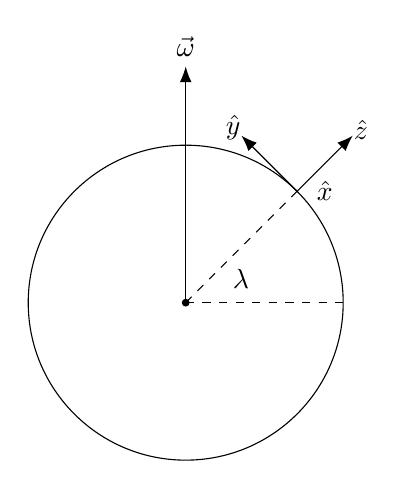
\begin{tikzpicture}
	\tikzmath{\t = 45; \r=2; \a=1.0;}
	\draw (0,0) circle (\r cm);
	\coordinate (A) at (\t:\r cm);
	\vectorin[3pt](A);
	
	\node[circle,fill=black,inner sep=1pt] at (0,0) {};
	%\draw (-0.4,2.5) edge[out=230,in=300,->,looseness=2.0] (0.4,2.6);
	\draw[->] (0,0) -- (0,3.0) node[anchor=south] {$\vec{\omega}$};
	\draw[dashed] (0,0) -- (\t:\r);
	\draw[dashed] (0,0) -- (\r, 0);
	\centerarc[](0,0)(0:\t:0.5);
	\node at (0.7, 0.3) {$\lambda$};
	\draw[->] (A) -- ($ (A) + (90+\t:\a) $) node[xshift=-3,yshift=3] {$\hat{y}$};
	\draw[->] (A) -- ($(A) + (\t:\a)$) node [xshift=3,yshift=2] {$\hat{z}$};
	\node[xshift=10] at (A) {$\hat{x}$};
	\end{tikzpicture}
\end{wrapfigure}
\begin{example}[Foucault pendulum]
		Consider a pendulum of length $ \ell $ and mass $m$, free to swing in the $(x,y)$ plane in the coordinates defined on the right. We ignore motion along $\hat{z}$. For the Earth, we also set $\dot{\vec{\omega}} = \vec{0}$. Now, note that the centrifugal force $\vec{\omega} \times (\vec{\omega} \times \vec{r})$ points along $ \hat{z} $. The net effect of this is to reduce the effective gravitational acceleration, so let $ g $ denote this reduced value. For small angles, the equation of motion with the Coriolis force is
		\[
			\ddot{r} = -\frac{g}{\ell} \vec{r} - 2 \vec{\omega} \times \dot{\vec{r}},
		\]
		where we ignore the $z$ component. Evaluating the cross product yields
		\begin{gather*}
			\ddot{x} - 2 \Omega \dot{y} + \frac{g}{\ell} x = 0, \\
			\ddot{y} + 2 \Omega \dot{x} + \frac{g}{\ell}y = 0,
		\end{gather*}
		where we defined $ \omega_z = \omega \sin \lambda = \Omega. $ We can rewrite this, defining $ u = x + iy $ as
		\[
		\ddot{u} + 2i \Omega \dot{u} + \omega_0^2 u = 0
		\]
		where $ \omega_0^ 2 = g/\ell $. The solution is given by
		\[
			u(t) = e^{-i\Omega t} \qty(A e^{i\omega_1 t} + B e^{-i \omega_1 t}),
		\]
		with $\omega_1 = \sqrt{\Omega^2 + \omega_0^2}$. Notice that $\Omega$ governs the rotation of the plane of swing.
	\end{example}
\subsection{Rotation about a fixed axis}
\begin{wrapfigure}{r}{0cm}
	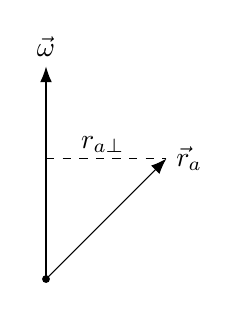
\begin{tikzpicture}[scale=0.9]
		\node[fill=black, circle, inner sep=1] at (0,0) {};
		\draw[->] (0,0) -- (0,3) node[anchor=south] {$\vec{\omega}$};
		\draw[->] (0,0) -- (1.7,1.7) node[anchor=west] {$\vec{r}_{a}$};
		\draw[dashed] (0,1.7) -- (1.7,1.7);
		\node at (0.8,1.9) {$r_{a\perp}$};
	\end{tikzpicture}
\end{wrapfigure}
First, let's consider the simple case where the direction of $ \vec{\omega} $ is fixed. Let $ \vec{\omega} $ point along $ \hat{e}_{3} $, so that $ \hat{e}_{3}(t) = \tilde{\hat{e}}_{3} $ for all $ t $. The total angular momentum along $ \hat{e}_{3} $ is
\begin{equation}
	L_{3} = \hat{e}_{3} \cdot \sum_{a} m_{a} \vec{r}_{a} \times (\vec{\omega} \times \vec{r}_{a}) = \sum_{a} m_{a} r_{a\perp}^{2} \omega = I \omega,
\end{equation}
where we defined the \textit{moment of inertia} about $ \hat{e}_{3} $ as $ I \defeq \sum_{a} m_{a} r_{a\perp}^{2} $, where $ r_{a\perp} $ is shown on figure to the right. The moment of inertia arises naturally from the kinetic energy as well:
\begin{gather}
	\begin{split}
		T = \frac{1}{2} \sum_{a} m_{a} \dot{\vec{r}}_{a} \cdot \dot{\vec{r}}_{a} & = \frac{1}{2} \sum_{a} m_{a} (\vec{\omega} \times \vec{r}_{a}) \cdot (\vec{\omega} \times \vec{r}_{a}) \\
		&= \frac{1}{2} \sum_{a} m_{a} \qty(\omega^{2} r_{a}^{2} - (\vec{\omega} \cdot \vec{r}_{a})^{2}) \\
		&= \frac{1}{2} \sum_{a} m_{a} \qty(r_{a}^{2} - (\vec{r}_{a} \cdot \hat{e}_{3})^2) \omega^{2} \\
		&= \frac{1}{2} \sum_{a} m_{a} r_{a\perp}^{2} \omega^{2} = \frac{1}{2} I \omega^{2},
	\end{split} 
\end{gather}
where note that $ r_{a\perp}^{2} = r_{a}^{2} - (\hat{e}_{3}\cdot \vec{r}_{a})^2 $. 
\subsubsection{Support force}
Suppose a free body rotates with some angular velocity $ \vec{\omega} $. Then, it follows that the body must rotate about its centre of mass, meaning $ \vec{\omega} $ should pass through the centre of mass position $ \vec{R} $. This is because, in the absence of external forces the centre of mass moves with constant velocity. In the frame of reference where the centre of mass is stationary, we must have
\begin{equation}
	\dot{\vec{R}} = \vec{\omega} \times \vec{R} = \vec{0} \implies \vec{\omega} \parallel \vec{R}.
\end{equation}
When the body doesn't rotate about its centre of mass, external forces are required to keep the rotation axis fixed. We write this condition as:
\begin{equation}
	\vec{F} + \vec{Q} = M \ddot{\vec{R}} = M \qty( \dot{\vec{\omega}} \times \vec{R} + \vec{\omega} \times (\vec{\omega} \times \vec{R}) + \vec{\omega} \times \vec{V}_{R} ),
\end{equation}
where $ \vec{V}_{R} $ denotes the centre of mass velocity as measured in the body frame. By definition, $ \vec{V}_{R} = \vec{0} $. $ \vec{F} $ is the net external force acting on the centre of mass of the body, and $ \vec{Q} $ is the support force acting through the rotation axis.  \\
\vspace{-0.5cm}
\begin{wrapfigure}{r}{0cm}
	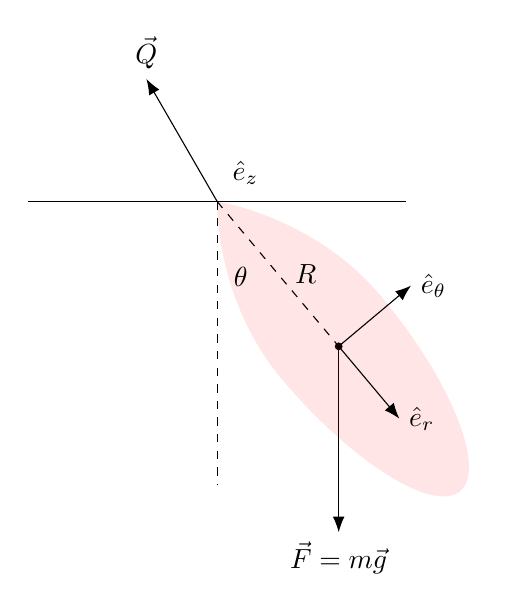
\begin{tikzpicture}[scale=1.2]
		\draw (-2,0) -- (2, 0);
		\node at (0.3,0.3) {$\hat{e}_{z}$};
		\node[fill=black, circle, inner sep = 1pt] at (310:2) {};
		\draw[->] (310:2) -- (2 * cos 310, -3.5) node[anchor=north]{$\vec{F} = m\vec{g}$};
		\fill[fill,red, fill opacity=0.1] plot [smooth, tension=1.0] coordinates {(0,0) (290:2) (310:4) (330:2) (0,0)};
		\draw[dashed] (0,0) -- (0,-3);
		\centerarc[](0,0)(270:310:0.7);
		\node at (0.25,-0.8) {$\theta$};
		\draw[dashed] (0,0) -- (310:1) node[xshift=10pt]{$R$} -- (310:2);
		\draw[->] (0,0) -- (120:1.5) node[anchor=south] {$\vec{Q}$};
		\draw[->] (310:2) -- (310:3) node[anchor=west] {$\hat{e}_{r}$};
		\draw[->] (310:2) -- ( $(310:2) + (40:1)$ ) node[anchor=west] {$\hat{e}_{\theta}$};
		\vectorout[1](0,0)
	\end{tikzpicture}
\end{wrapfigure}
\begin{example}[Compound pendulum]
	Consider a compound pendulum with moment of inertia of $ I $ about $ \hat{e}_{z} $ and mass $m$ with centre of mass a distance $R$ away from the pivot. The equation of motion is:
	\[
		\ddot{\theta} = \frac{mgR}{I} \sin \theta,
	\]
	along with energy conservation:
	\[
		\frac{1}{2} I \dot{\theta}^{2} - mg R \cos \theta = E.
	\]
	Note that $ \vec{\omega} = \dot{\theta} \hat{e}_{z} $ and $ \vec{R} = R \hat{e}_{r} $. Then, the inertial forces are:
	\[
	\dot{\vec{\omega}} \times \vec{R} = R \ddot{\theta}  \, \hat{e}_{\theta}, \quad
	\vec{\omega} \times (\vec{\omega} \times \vec{R}) = - R \dot{\theta}^{2} \hat{e}_{r}.
	\]
	Finally, in the body frame the external force is
	\[
		\vec{F} = mg \qty( \cos \theta \, \hat{e}_{r} - \sin \theta \, \hat{e}_{\theta} ).
	\]
	Putting everything together and substituting for $ \dot{\theta} $ and $ \ddot{\theta} $, we find that the support force is
	\[
		\vec{Q} = mg \sin \theta \qty(1 - \frac{mR^2}{I}) \, \hat{e}_{\theta} - \qty(mg\cos\theta \qty[1 + \frac{2mR^2}{I}] + \frac{2mR}{I} E) \, \hat{e}_{r}.
	\]
	This does not necessarily act radially, as the $ \hat{e}_{\theta} $ component is non-zero for $ I \neq mR^{2} $.
\end{example}
\subsection{Inertia tensor}
The inertia tensor generalises the moment of inertia to rotations about arbitrary axes. It again arises naturally from the angular momentum and kinetic energy. The angular momentum is
\begin{align}
    \begin{split}
        \vec{L} = \sum_i m_i \vec{r}_i \times \dot{\vec{r}}_i &= \sum_i m_i \vec{r}_i \times \qty(\vec{\omega} \times \vec{r}_i) \\
        &= \sum_i m_i \hat{e}_a \epsilon_{abc} r_{i,b} \epsilon_{cde} \omega_d r_{i,e} \\
        &= \hat{e}_a \sum_i m_i \qty(\delta_{ad}\delta_{be} - \delta_{ae}\delta_{bd}) r_{i,b} \omega_d r_{i,e} \\
        &= \hat{e}_a \sum_i m_i \qty(r_i^2 \omega_a - r_{i,a} r_{i,b} \omega_b) \\
        &= \hat{e}_a \sum_i m_i \qty(r_i^2 \delta_{ab} - r_{i,a} r_{i,b}) \omega_b.
    \end{split}
\end{align}
Hence, we see that the components of $\vec{L}$ are
\begin{equation}
    L_a = \sum_i m_i \qty(r_i^2 \delta_{ab} - r_{i,a} r_{i,b}) \omega_b \equiv I_{ab} \omega_b,
\end{equation}
where we defined the \href{https://en.wikipedia.org/wiki/Moment_of_inertia#Inertia_tensor}{\textit{inertia tensor}} $I$ with components
\begin{equation} \label{inertiatensor}
    I_{ab} \defeq \sum_i m_i \qty(r_i^2 \delta_{ab} - r_{i,a} r_{i,b}).
\end{equation}
Now, consider the kinetic energy:
\begin{align}
    \begin{split}
        T = \frac{1}{2} \sum_i m_i \dot{\vec{r}}_i \cdot \dot{\vec{r}}_i &= \frac{1}{2} \sum_i m_i \qty(\vec{\omega} \times \vec{r}_i) \cdot \qty(\vec{\omega} \times \vec{r}_i) \\
        &= \frac{1}{2} \sum_i m_i \qty(\epsilon_{abc} \omega_b r_{i,c}) \qty(\epsilon_{ade}\omega_d r_{i,e}) \\
        &= \frac{1}{2} \sum_i m_i \qty(\delta_{bd}\delta_{ce} - \delta_{be}\delta_{cd}) \omega_b \omega_d r_{i,c} r_{i,e} \\
        &= \frac{1}{2} \sum_i m_i \qty(r_i^2 \delta_{bc} - r_{i,c} r_{i,b}) \omega_b \omega_c \\
        &= \frac{1}{2} \omega_b I_{bc} \omega_c = \frac{1}{2} \vec{\omega} \cdot I \vec{\omega}.
    \end{split}
\end{align}
From the definition of the inertia tensor \eqref{inertiatensor}, it follows that $I$ is symmetric:
\begin{equation}
    I_{ab} = \sum_i m_i \qty(r_i^2 \delta_{ab} - r_{i,a} r_{i,b}) = \sum_i m_i \qty(r_i^2 \delta_{ba} - r_{i,b} r_{i,a}) = I_{ba}.
\end{equation}
The components of the inertia tensor are measured in the body frame because we used the relation \eqref{rotatingframe2}. Since the components of the position vector $r_i$ are time-independent in the body frame, so are the components of $I$. 
\par
The inertia tensor generalizes to continuous bodies as follows:
\begin{equation} \label{eq:inertiatensor}
    I = \int \dd[3]{r} \rho(\vec{r}) \mqty(y^2+z^2 & -xy & -xz \\ -yx & z^2 + x^2 & -yz \\ -zx & -zy & x^2 + y^2),
\end{equation}
where we denote the position vector in the body frame as
\[
    \vec{r} = x \hat{e}_1 + y \hat{e}_2 + z \hat{e}_3.
\]
Since the inertia tensor is a real, symmetric matrix, we can diagonalise it by an \href{https://en.wikipedia.org/wiki/Orthogonal_transformation}{orthogonal transformation}: $I' = O I O^T$ and $\hat{e}'_a = O \hat{e}_a$ where $O$ is an orthogonal matrix. This would yield
\begin{equation}
    I = \mqty(\dmat{I_1, I_2, I_3}).
\end{equation}
The body axes in which $I$ is diagonal are called the \href{https://en.wikipedia.org/wiki/Moment_of_inertia#Principal_axes}{\textit{principal axes}}. Eigenvalues $I_{1,2,3}$ are called the \textit{principal moments.} The angular momentum and kinetic energy take particularly simple forms under this choice of axes:
\begin{equation}
    \vec{L} = I_1 \omega_1 \hat{e}_1 + I_2 \omega_2 \hat{e}_2 + I_3 \omega_3 \hat{e}_3 \qq{and} T = \frac{1}{2}\qty(I_1 \omega_1^2 \hat{e}_1 + I_2 \omega_2^2 \hat{e}_2 + I_3 \omega_3^2 \hat{e}_3).
\end{equation}
\par
If any two principal moments are equal, $ I_{i} = I_{j} $, then the body is said to be \textit{symmetric}. Then, any two perpendicular vectors lying in the plane spanned by $ \hat{e}_{i} $ and $ \hat{e}_{j} $ are also principal axes. To see why, set $ I_{2} = I_{3} $ and consider a rotation by angle $ \theta $ around $ \hat{e}_{1} $:
\[
	I' = OIO^T = \mqty(1 & 0 & 0 \\ 0 & \cos \theta & \sin \theta \\ 0 & -\sin\theta & \cos \theta)  \mqty(\dmat{I_1, I_2, I_2}) \mqty(1 & 0 & 0 \\ 0 & \cos \theta & -\sin \theta \\ 0 & \sin\theta & \cos \theta) =  \mqty(\dmat{I_1, I_2, I_2}) = I.
\]
If all principal moments are equal, the body is said to be \textit{totally symmetric}. In this case, any three mutually orthonormal vectors are principal axes. 
\\\\
\begin{wrapfigure}{r}{0cm}
	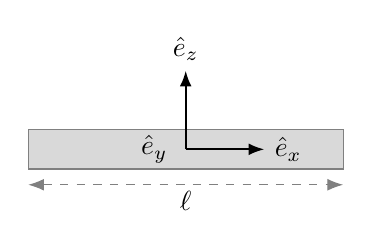
\begin{tikzpicture}[scale=1] % rigid rod
	\tikzmath{\e = 1.0; \l = 2; \h=0.25;}
	\colorlet{mycolor}{black!15}
	\draw[fill, color=mycolor] (-\l, -\h) rectangle (\l, \h); 
	\draw[color=gray] (-\l, -\h) rectangle (\l, \h);
	\coordinate (O) at (0, 0);
	\node at (-0.4,0) {$\hat{e}_{y}$};
	\draw[thick, ->] (O) -- (\e, 0) node[anchor=west] {$\hat{e}_{x}$};
	\draw[thick, ->] (O) -- (0, \e) node[anchor=south] {$\hat{e}_{z}$};
	\vectorin[3pt](0,0)
	\draw[<->, dashed, gray] (-\l, -\h-0.2) -- (\l, -\h-0.2);
	\node at (0, -\h-0.4) {$\ell$} ;
	\end{tikzpicture}
\end{wrapfigure}
\vspace{-1cm}
\subsubsection{Examples}
\begin{example}[Rigid rod]
	Consider a rigid, one dimensional rod of mass $ m $ with length $\ell$ along $ \hat{e}_x $, as shown on the figure. The centre of mass is located at the origin. The mass density is
	\[
	\rho(\vec{r}) = \begin{cases}
	m / \ell & y = z = 0, \, \abs{x} \leq \ell/2, \\
	0 & \text{otherwise.}
	\end{cases}
	\]
	Setting $ y = z = 0 $ in equation \eqref{eq:inertiatensor} yields $ I_{11} = 0 $, $ I_{ij} = 0 $ for all $ i \neq j $, and
	\[
	I_{22} = I_{33} = \int_{-\ell/2}^{\ell/2} \dd{x} \frac{m}{\ell} x^{2} = \frac{m \ell^{2}}{12}.
	\]
	The body is symmetric, as we would expect. Since the body has no extension along $ \hat{e}_{y} $ or $ \hat{e}_z $, the principal moment along $ \hat{e}_{x} $ is zero. As all non-diagonal terms in $ I $ are zero, $ \hat{e}_{x,y,z} $ are principal axes.
\end{example}
\begin{figure}[h]
	\centering
	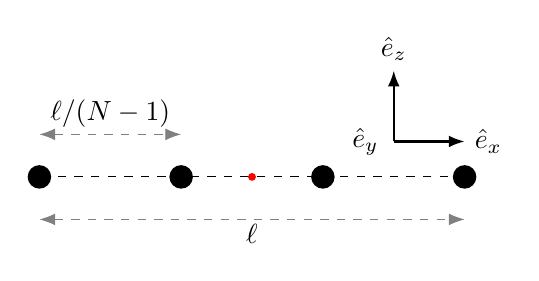
\begin{tikzpicture}[scale=0.9] % line of beads
	\tikzmath{\e = 1.0; \n = 4; \l = 6;}
	\foreach \i in {1,...,\n}
	\node[fill, circle, inner sep=3] at ({ (\i-1)*\l / (\n-1) - \l/2},0) {};
	\coordinate (O) at (0, 0);
	\coordinate (A) at (\l/2-\e, 0.5);
	\node at ($(A)+(-0.4,0)$) {$\hat{e}_{y}$};
	\draw[dashed] (\l/2,0) -- (-\l/2,0);
	\draw[thick, ->] (A) -- +(\e, 0) node[anchor=west] {$\hat{e}_{x}$};
	\draw[thick, ->] (A) -- +(0, \e) node[anchor=south] {$\hat{e}_{z}$};
	\vectorin[3pt](A)
	\draw[<->, dashed, gray] (-\l/2, -0.6) -- (\l/2, -0.6);
	\node at (0, -0.8) {$\ell$} ;
	\draw[<->, dashed, gray] (-\l/2, 0.6) -- ({-\l/2 + 1/(\n-1) * \l}, 0.6);
	\node at (-\l/2+1.0, 0.9) {$\ell / (N-1)$};
	\node[fill, circle, inner sep = 1, color=red] at (0,0) {};
	\end{tikzpicture}
\end{figure}
\begin{example}[Line of beads]
	Consider a line of $ N $ equidistant beads of equal mass along the $ x $ axis as shown on the figure. Enumerate beads by $ i = 1, \dots, N $ so that the position of the $ i $-th bead is
	\[
		x_{i} = -\frac{\ell}{2}	+ \frac{\ell (i-1)}{(N-1)}, \quad y_{i} = z_{i} = 0.
	\]
	The inertia tensor is
	\[
		I = \sum_{i = 1}^{N} \frac{M}{N} \mqty( 0 & 0 & 0 \\ 0 & x_{i}^{2} & 0 \\ 0 & 0 & x_{i}^{2} )
	\]
	where $ M $ is the total mass. By symmetry, we again have $ I_{22} = I_{33} $. Performing the sum yields
	\[
	I_{22} = I_{33} = M \ell^{2} \qty( \frac{2N-1}{6(N-1)} - \frac{1}{4} ).
	\]
	As a sanity check, note that this is always positive for $ N \geq 2 $. Furthermore, in the limit $ N \to \infty $, we recover the moment for rigid rod.
\end{example}
\begin{figure}[h]
	\centering
	\begin{tikzpicture}[scale=1.5, tdplot_main_coords] % cube
	\tikzmath{\a = 1.0;}
	\coordinate (O) at (0, 0, 0);
	\draw (\a,\a,\a) -- (-\a,\a,\a) -- (-\a,\a,-\a) -- (\a,\a,-\a) -- cycle;
	\draw (\a,\a,\a) -- (\a,-\a,\a) -- (\a,-\a,-\a) -- (\a,\a,-\a);
	\draw(\a,-\a,\a) -- (-\a,-\a,\a) -- (-\a,\a,\a);
	\draw[dashed] (-\a,-\a,\a) -- (-\a,-\a,-\a) -- (-\a, \a, -\a);
	\draw[dashed] (-\a,-\a,-\a) -- (\a,-\a,-\a);
	\shade[left color = gray!70, right color= gray!70, opacity = 0.5] (\a,\a,\a) -- (-\a,\a,\a) -- (-\a,\a,-\a) -- (\a,\a,-\a) -- cycle;
	\shade[top color = white, right color = gray!60, opacity = 0.5] (\a,\a,\a) -- (\a,-\a,\a) -- (\a,-\a,-\a) -- (\a,\a,-\a);
	\shade[left color = white, right color= gray!60, opacity = 0.5] (\a,-\a,\a) -- (-\a,-\a,\a) -- (-\a,\a,\a) -- (\a,\a,\a);
	\draw[thick,->] (0,0,0) -- (1,0,0) node[anchor=north]{$\hat{e}_{x}$}; 
	\draw[thick,->] (0,0,0) -- (0,1,0) node[anchor= west]{$\hat{e}_y$};
	\draw[thick,->] (0,0,0) -- (0,0,1) node[anchor=south]{$\hat{e}_{z}$};
	\node[fill, circle, inner sep = 1] at (O) {};
	\draw[dashed, <->, gray] (\a, -\a, -\a-0.2) -- (\a, \a, -\a-0.2);
	\node at (\a, 0, -\a-0.4) {$a$};
	\end{tikzpicture}
	\hspace{1cm}
	\begin{tikzpicture}[scale=1.5, tdplot_main_coords] % sphere
	\tikzmath{\r = 1.5; \e = 1.0;}
	\tdplotsetrotatedcoords{-30}{0}{0};
	\coordinate (O) at (0, 0, 0);
	\shadedraw[ball color = gray!20, opacity=0.4] (O) circle (\r cm);
	\draw[dashed, color=gray] (0,0,0) circle (\r);
	\draw[thick,->,tdplot_rotated_coords] (0,0,0) -- (\e,0,0) node[anchor=north]{$\hat{e}_{x}$}; 
	\draw[thick,->,tdplot_rotated_coords] (0,0,0) -- (0,\e,0) node[anchor= west]{$\hat{e}_y$};
	\draw[thick,->,tdplot_rotated_coords] (0,0,0) -- (0,0,\e) node[anchor=south]{$\hat{e}_{z}$};
	\node[fill, circle, inner sep = 1] at (O) {};
	\draw[<->, gray, dashed,tdplot_rotated_coords] (O) -- (0, -\r, 0);
	\node[tdplot_rotated_coords] at (0, -\r / 2 + 0.2, 0.2) {$a$};
	\end{tikzpicture}
\end{figure}
\begin{example}[Cube]
	Consider cube of side length $ a $ and total mass $ M $. The mass distribution is uniform:
	\[
		\rho(\vec{r}) = \begin{cases} 
		\flatfrac{M}{a^{3}} & (x,y,z) \in \qty[\flatfrac{-a}{2}, \flatfrac{a}{2}]^{3}, \\ 0 & \text{otherwise}.
		\end{cases}
	\]
	It is obvious by symmetry that $ I_{11} = I_{22} = I_{33}$:
	\[
		I_{33} = \frac{M}{a^{3}} \int_{-a/2}^{a/2} \dd{x} \int_{-a/2}^{a/2} \dd{y} \int_{-a/2}^{a/2} \dd{z} (x^{2} + y^{2}) = \frac{2M}{a} \int_{-a/2}^{a/2} \dd{x} x^{2} = \frac{M a^{2}}{6}.
	\]
	The cross terms evaluate to zero since the integrands are odd. The body is totally symmetric.
\end{example}
\begin{example}[Sphere]
	Consider a sphere with radius $ a $, total mass $ M $. The mass distribution is uniform:
	\[
		\rho(\vec{r}) = \begin{cases}
		\flatfrac{3M}(4 \pi a^{3}) & x^{2} + y^{2} + z^{2} \leq a, \\ 0 & \text{otherwise.}
		\end{cases}
	\]
	Clearly, by symmetry $ I_{11} = I_{22} = I_{33} $: 
	\[
		I_{33} = \frac{3 M}{4 \pi a^{3}} \int_{\vec{r}^{\,2} \leq a} \dd{\vec{r}} (x^{2} + y^{2}) = \frac{2}{5} M a^{2}.
	\]
	Likewise, the cross terms evaluate to zero due to symmetry. The body is totally symmetric. 
	\par
	Here is a fun thought experiment: Consider two free masses, a cube with side length $ \ell $ and a sphere of radius $ \sqrt{\flatfrac{5}{12}} \ell$. How can we tell them apart if we can only probe their rotational and translational degrees of freedom?
\end{example}
\subsubsection{Parallel axis theorem}
So far, we have only been calculating the inertia tensor about the centre of mass. If the body is not free, it will not necessarily rotate about its centre of mass. But the inertia tensor about the centre of mass has a nice property which allows us to compute the inertia tensor about an arbitrary point more easily. We write the position vector as $\vec{r}_i = \vec{r}_i^{\,*} + \vec{R}$, where $\vec{R}$ is the centre of mass position. Then, the inertia tensor is
\begin{align}
    \begin{split}
        I_{ab} =& \sum_i m_i \qty(r_i^2 \delta_{ab} - r_{i,a} r_{i,b}) \\
        =& \sum_i m_i \qty(\qty[\vec{r}_i^{\,*} + \vec{R}]^2 \delta_{ab} - (r_{i,a}^{\,*} + R_a)({r}_{i,b}^{\,*} + R_b) ) \\
        =& \sum_i m_i \qty(\qty[(r^{\,*}_i)^2 + 2 r_i^{\,*}R + R^2]\delta_{ab} - {r}_{i,a}^{\,*}{r}_{i,b}^{\,*} - {r}_{i,a}^{\,*}R_b - R_a {r}_{i,b}^{\,*} - R_a R_b ) \\
        =&  \sum_i m_i \qty(({r}_{i}^{\,*})^2\delta_{ab} - {r}_{i,a}^{\,*}{r}_{i,b}^{\,*}) + 2R\delta_{ab} \underbrace{\sum_i m_i r_i^{\,*}}_{\equiv 0} - R_b \underbrace{\sum_i m_i r_{i,a}^*}_{\equiv 0} - R_a \underbrace{\sum_i m_i r_{i,b}^*}_{\equiv 0} \\&+ \sum_i m_i \qty(R^2 \delta_{ab} - R_a R_b) \\
        =& I^*_{ab} + M \qty(R^2 \delta_{ab} - R_a R_b).
    \end{split}
\end{align}
So the inertia tensor decouples into the inertia tensor about the centre of mass $I^*$ and the inertia tensor of the centre of mass. This is known as the \href{https://en.wikipedia.org/wiki/Parallel_axis_theorem}{\textit{parallel axis theorem.}}
\subsection{Euler's equations}
We are interested the equation of motion for a rotating rigid body under external torque $\vec{\tau}$. As we can completely specify the rotation of the body by the rotation matrix $R(t)$, and since it is possible to obtain $R(t)$ from $\vec{\omega}(t)$, we may look for an equation relating $\vec{\omega}$ to $\vec{\tau}$. We start by stating
\begin{equation}
    \dv{\vec{L}}{t} = \dv{}{t}\qty(L_a \hat{e}_a) = \dot{L}_a \hat{e}_a + L_a \vec{\omega} \times \hat{e}_a = \vec{\tau}.
\end{equation}
Now, we work in the principal axes and write the principal moments as $I^{(1,2,3)}$ to avoid confusion with the summation convention. Then, we have $L_a = I^{(a)} \omega_a$ and so
\begin{equation}
    \dot{\vec{L}} = I^{(a)} \dot{\omega}_a \hat{e}_a + I^{(a)} \omega_a \omega_b \hat{e}_b \times \hat{e}_a = I^{(a)} \dot{\omega}_a \hat{e}_a + I^{(a)} \omega_a \omega_b \epsilon_{bac} \hat{e}_c.
\end{equation}
Substituting this yields
\begin{gather}
    \dot{\vec{L}} = \qty(I^{(c)} \dot{\omega}_c + I^{(a)} \omega_a \omega_b \epsilon_{bac}) \hat{e}_c = \vec{\tau} \\
    \implies \dot{L}_c = I^{(c)} \dot{\omega}_c + \epsilon_{cba} \omega_a \omega_b I^{(a)} = \tau_c.
\end{gather}
We may explicitly write the set of three equations:
\begin{gather}
    \dot{L}_1 = I^{(1)} \dot{\omega}_1 + \omega_2 \omega_3 \qty(I^{(3)} - I^{(2)}) = \tau_1, \\
    \dot{L}_2 = I^{(2)} \dot{\omega}_2 + \omega_3 \omega_1 \qty(I^{(1)} - I^{(3)}) = \tau_2, \\
    \dot{L}_3 = I^{(3)} \dot{\omega}_3 + \omega_1 \omega_2 \qty(I^{(2)} - I^{(1)}) = \tau_3.
\end{gather}
These are called the \textit{Euler equations.}
\subsection{Euler angles}
We want an explicit parametrisation of the rotation which takes us from the space to the body frame. Any arbitrary rotation may be expressed as a composition of 3 rotations about 3 different axes. We want rotation $R$ such that $\hat{e}_a = R_{ab} \tilde{\hat{e}}_b$. Let's split this into the three steps:
\begin{equation}
    \{\tilde{\hat{e}}_a\} \xrightarrow{R_3(\phi)} \{\hat{e}'_a\} \xrightarrow{R_1(\theta)} \{\hat{e}''_a\} \xrightarrow{R_3(\psi)} \{\hat{e}_a\}.
\end{equation}
First, we rotate by $\phi$ about $\tilde{\hat{e}}_3$. So, $\hat{e}_a' = R_3(\phi)_{ab}\tilde{\hat{e}}_b$ where
\begin{equation}
    R_3(\phi) = \mqty(\cos\phi & \sin\phi & 0 \\ -\sin\phi & \cos\phi & 0 \\
    0 & 0 & 1).
\end{equation}
Then, we rotate by $\theta$ around $\hat{e}'_1$ so that $\hat{e}_a'' = R_1(\theta)_{ab} \hat{e}_b'$, where
\begin{equation}
    R_1(\theta) = \mqty(1 & 0 & 0 \\ 0 & \cos \theta & \sin \theta \\ 0 & -\sin\theta & \cos \theta).
\end{equation}
Finally, we rotate by $\psi$ about $\hat{e}_3''$ so that $\hat{e}_a = R_3(\psi)_{ab} \hat{e}_b''$ where
\begin{equation}
    R_3(\psi) = \mqty(\cos\psi & \sin\psi & 0 \\ -\sin\psi & \cos\psi & 0 \\
    0 & 0 & 1).
\end{equation}
Putting everything together, we have $R(\phi,\theta,\psi) = R_3(\psi)R_{1}(\theta)R_3(\phi)$.
\par
Let's now express the angular velocity in terms of the Euler angles $\phi,\theta,\psi$. In time $\dd{t}$, the angles change as
\[
    (\phi, \theta, \psi) \longrightarrow (\phi + \dd{\phi}, \theta + \dd{\theta}, \psi + \dd{\psi}),
\]
which means the angular displacement is
\[
    \vec{\omega}\dd{t} = \dd{\phi} \tilde{\hat{e}}_3 + \dd{\theta} \hat{e}_1' + \dd{\psi} \hat{e}_3'',
\]
and hence the angular velocity is given by
\begin{equation}
    \vec{\omega} = \dot{\phi}\, \tilde{\hat{e}}_3 + \dot{\theta}\,\hat{e}'_1 + \dot{\psi}\, \hat{e}_3''.
\end{equation}
Now, we need to write $\tilde{\hat{e}}_3, \hat{e}_1'$ and $\hat{e}_3''$ in terms of $\hat{e}_{1,2,3}$. This is a straightforward computation:
\begin{gather*}
    \hat{e}_3'' = \hat{e}_3, \\
    \hat{e}_1' = \hat{e}_1'' = \cos\psi \, \hat{e}_1 - \sin\psi\, \hat{e}_2, \\
    \tilde{\hat{e}}_3 = \hat{e}_3' = \sin\theta \, \hat{e}_2'' + \cos\theta \, \hat{e}_3'' = \sin\theta (\sin\psi \, \hat{e}_1 + \cos\psi \, \hat{e}_2) + \cos \theta \,\hat{e}_3.
\end{gather*}
Hence, we have
\begin{align}
    \begin{split}
        \vec{\omega} &= \dot{\phi} \qty(\sin\theta (\sin\psi \, \hat{e}_1 + \cos\psi \, \hat{e}_2) + \cos \theta \,\hat{e}_3) + \dot{\theta} \qty(\cos\psi \, \hat{e}_1 - \sin\psi\, \hat{e}_2) + \dot{\psi} \, \hat{e}_3 \\
        &= \hat{e}_1 \qty(\dot{\phi} \sin\theta \sin \psi + \dot{\theta} \cos\psi) + \hat{e}_2 \qty(\dot{\phi} \sin\theta \cos\psi - \dot{\theta} \sin\psi) + \hat{e}_3 \qty(\dot{\phi} \cos\theta + \dot{\psi}).
    \end{split}
\end{align}

\newpage

\section{Lagrangian Mechanics}
\textit{(We use Einstein summation convention throughout this chapter.)}
\subsection{Generalised coordinates}
Newton's laws restrict us to deal with components of vectors in inertial frames. We are interested in formulating classical mechanics in a way more general than that. A sensible first step would be to propose a way of specifying the configuration of a system.
\par
The (spatial) configuration of any given system with (finite) $N$ degrees of freedom is specified by a finite set of coordinates $\{q^1, q^2, \dots, q^N \}$.\footnote{Strictly speaking, the configuration of a system at a given time is represented by a point on an $ N $ dimensional manifold. The coordinate functions $ q^{i} $ provide a local chart to the manifold. To specify the complete state of the system, we need to specify velocities associated to each coordinate. This corresponds to the tangent bundle of the manifold,  which itself is a $ 2N $ dimensional manifold. The same information is captured by the cotangent bundle. It is called the \textit{phase space}.} Such a set of coordinates is called \textit{generalised coordinates.} For example, a set of $n$ free particles requires $3n$ generalised coordinates to specify the position of each. A free rigid body is described by $6$ coordinates: 3 for centre of mass position and 3 Euler angles. 
\par
We can go one step further and define a \textit{configuration space} $\mathcal{C}$ as the space of all possible configurations of the system. A choice of generalised coordinates $\{q^a\}$ then becomes an explicit parametrisation of $\mathcal{C}$. The configuration of a system at any given time corresponds to a \textit{point} in $\mathcal{C}$. As the system evolves in time, it traces out a \textit{curve} in $\mathcal{C}$.
\par
All we need now is a method to determine which particular curve is traversed.
\subsection{Action principle}
Since we are interested in finding a particular curve out of all possible curves in the configuration space, we will need to use \textit{variational calculus.} Let's define a \textit{functional} of the generalised coordinates such that a stationary point of the functional corresponds to the path traversed in the configuration space. This functional $\mathcal{S}[q]$, called the \href{https://en.wikipedia.org/wiki/Action_(physics)}{\textit{action}}, is defined as
\begin{equation} \label{action}
    \mathcal{S}[q] \defeq \int_{t_i}^{t_f} L(q,\dot{q},t) \dd{t},
\end{equation}
where $L(q,\dot{q},t)$\footnote{The set of all generalised coordinates $\{q^1, \dots, q^N\}$ is denoted by $q$, and similarly $\dot{q}$ denotes the set $\{\dot{q}^1,\dots,\dot{q}^N\}$.} is the \textit{Lagrangian}, defined as the difference between the kinetic and potential energy of the system:
\begin{equation}
    L(q,\dot{q},t) \defeq T(\dot{q}) - V(q,t).
\end{equation}
Out of all curves in $\mathcal{C}$ with fixed endpoints
\begin{equation}\label{variationboundary}
    q(t_i) = q_{i} \qq{and} q(t_f) = q_{f},
\end{equation}
the system follows the one which makes the action $\mathcal{S}$ stationary. This is called the \textit{action principle}.
\par
Note that in equation \eqref{action} we assumed that the curve is parametrised by time so that $q^a = q^a(t)$. Equivalently, we could have used an arbitrary parametrisation. If the Lagrangian has explicit time dependence, using another parametrisation would imply that time itself should be taken as a generalised coordinate. In relativity, since space and time are treated on an equal footing, the curve may not always be parametrised by time.
\subsection{Euler-Lagrange equations}
To find the path which stationarises the action, we consider the variation
\begin{equation}
    \delta \mathcal{S} = \mathcal{S}[q + \delta q] - \mathcal{S}[q],
\end{equation}
where $\delta q$ is a small perturbation to the trajectory. The boundary condition \eqref{variationboundary} implies
\begin{equation}
    \delta q(t_i) = \delta q(t_f) \equiv 0.
\end{equation}
The variation in the Lagrangian is
\begin{equation}
    \delta L = L(q+\delta q, \dot{q} + \delta \dot{q}, t) - L(q,\dot{q},t) = \pdv{L}{q^a} \delta q^a + \pdv{L}{\dot{q}^a}\delta \dot{q}^a.
\end{equation}
Note that we always work up to linear order in $ \delta q $. The variation in the action is then given by
\begin{equation}
    \delta \mathcal{S} = \int_{t_i}^{t_f} \delta L\dd{t} = \int_{t_i}^{t_f} \qty(\pdv{L}{q^a} \delta q^a + \pdv{L}{\dot{q}^a}\delta \dot{q}^a) \dd{t}.
\end{equation}
Integrating second term by parts:
\[
    \int_{t_i}^{t_f} \pdv{L}{\dot{q}^a} \delta \dot{q} \dd{t} = \underbrace{\pdv{L}{\dot{q}^a} \delta q^a \eval_{t_i}^{t_f}}_{=0} - \int_{t_i}^{t_f} \dv{}{t}\qty(\pdv{L}{\dot{q}^a}) \delta q^a \dd{t} = - \int_{t_i}^{t_f} \dv{}{t}\qty(\pdv{L}{\dot{q}^a}) \delta q^a \dd{t}.
\]
Hence, we have
\begin{equation}
    \delta \mathcal{S} = \int_{t_i}^{t_f} \qty[\pdv{L}{q^a} - \dv{t}\qty(\pdv{L}{\dot{q}^a})] \delta q^a \dd{t} = 0.
\end{equation}
Since this must hold for all $\delta q$, we must have
\begin{equation}
    \pdv{L}{q^a} - \dv{t}\qty(\pdv{L}{\dot{q}^a}) = 0 \quad \forall \, a.
\end{equation}
This is known as the \href{https://en.wikipedia.org/wiki/Action_(physics)#Euler–Lagrange_equations_for_the_action_integral}{\textit{Euler-Lagrange equation}}. 
\par
As a side note, the \href{https://en.wikipedia.org/wiki/Functional_derivative}{\textit{functional derivative}} $\fdv*{\mathcal{S}}{q}$ is defined such that
\begin{equation}
    \delta \mathcal{S} = \int \fdv{\mathcal{S}}{q^a} \delta q^a \dd{t}.
\end{equation}
So, for a Lagrangian which depends on $q, \dot{q}$ and $t$, the functional derivative is
\begin{equation}
    \fdv{\mathcal{S}}{q^a} = \pdv{L}{q^a} - \dv{}{t} \qty(\pdv{L}{\dot{q}^a}).
\end{equation}
\par
We may now show that the action principle is equivalent to Newton's laws. Choosing Cartesian coordinates, we have
\[
    T = \frac{1}{2} m (\dot{x}^2 + \dot{y}^2 + \dot{z}^2)
\]
for a single particle. Then,
\begin{equation} \label{eq:lagrangenewton}
    \pdv{L}{x^a} - \dv{t}\qty(\pdv{L}{\dot{x}^a}) =  - m \ddot{x}_a - \pdv{V}{x^a} = 0 \implies m \ddot{\vec{x}} = -\grad{V}.
\end{equation}
\begin{figure}%{r}{0cm}
	\centering
	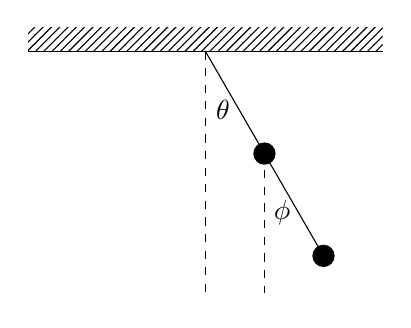
\begin{tikzpicture}[scale=1.5]
	\fill [pattern = north east lines] (-1.5,0) rectangle (1.5,0.2);
	\draw[dashed] (0,0) -- (0,-2.1);
	\draw (-1.5,0) -- (1.5,0);
	\draw (0,0) -- (-60:1) node[circle,fill=black,inner sep=1mm] {};
	\draw (-60:1) -- +(-60:1) node[circle,fill=black,inner sep=1mm] {};
	\draw[dashed] (-60:1) -- +(0,-1.18);
	\node at (0.15,-0.5) {$ \theta $};
	\node at ($(0.15,-0.5)+(-60:1)$) {$ \phi $};
	\end{tikzpicture}
	\hspace{1cm}
	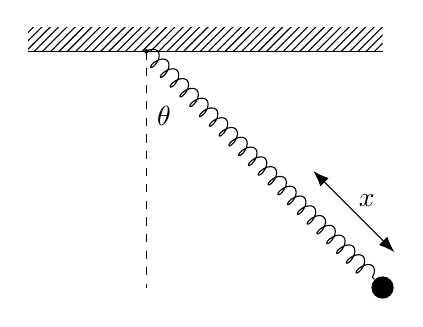
\begin{tikzpicture}[scale=1.5] % spring pendulum
	\node[circle,fill=black,inner sep=1mm] (a) at (2,-2) {};
	\node[circle, fill=black, inner sep=0.2mm] at (0,0) {};
	\draw[decoration={aspect=0.5, segment length=5, amplitude=3,coil},decorate] (0,0) -- (a); 
	\fill [pattern = north east lines] (-1,0) rectangle (2,0.2);
	\draw (-1,0) -- (2,0);
	\draw[dashed] (0,0) -- (0,-2);
	\node at (0.15,-0.55) {$ \theta $};
	\draw [<->] ([yshift=0.4cm]-45:2) -- ([yshift=0.4cm]-45: {2.1 * sqrt(2)}) node[xshift=-0.35cm, yshift=0.65cm] {$x$};
	\end{tikzpicture}
\end{figure}
\begin{example}[Double pendulum]
	Consider two equal point masses $ m $ attached with rigid rods of length $ \ell $ as shown from the figure. The system admits a two dimensional configuration space spanned by $ (\theta, \phi) \in [0,2\pi)^{2} $ (as a manifold, this is a torus). The kinetic energy and potential energies are
	\begin{gather*}
		T = m \ell^{2} \dot{\theta}^{2} + \frac{1}{2} m \ell^{2} \dot{\phi}^{2} + m \ell^{2} \dot{\theta} \dot{\phi} \cos(\theta - \phi), \\
		V = - mg\ell \qty(2\cos\theta + \cos \phi).
	\end{gather*}
	Hence, the Lagrangian:
	\[
		L = T - V = m \ell^{2} \dot{\theta}^{2} + \frac{1}{2} m \ell^{2} \dot{\phi}^{2} + m \ell^{2} \dot{\theta} \dot{\phi} \cos(\theta - \phi) + mg\ell \qty(2\cos\theta + \cos \phi).
	\]
	The Euler-Lagrange equations for $ \theta $ and $ \phi $ are
	\begin{gather*}
		2\ell \ddot{\theta} + \ell \ddot{\phi} \cos(\theta - \phi) + \ell \dot{\phi}^{2} \sin(\theta - \phi) + 2g \sin \theta = 0, \\
		\ell \ddot{\phi} + \ell \ddot{\theta} \cos(\theta - \phi) - \ell \dot{\theta}^{2} \sin(\theta - \phi) + g \sin \phi = 0.
	\end{gather*}
	These form a system of coupled second-order nonlinear differential equations. 
\end{example}
\begin{example}[Spring pendulum]
	Consider point mass $ m $ and let $ \theta $ denote the angle from the vertical and $ x $ the extension of the spring, $ \ell $ the natural length of the spring, and $ k $ the spring constant. Then, we can write the kinetic and potential energy:
	\begin{gather*}
		T = \frac{1}{2} m (\ell + x)^{2} \dot{\theta}^{2} + \frac{1}{2} m \dot{x}^{2} \\
		V = - mg (\ell + x) \cos \theta  + \frac{1}{2} k x^{2}.
	\end{gather*}
	The Lagrangian is
	\[
		L = T - V = \frac{1}{2} m (\ell + x)^{2} \dot{\theta}^{2} + \frac{1}{2} m \dot{x}^{2} + mg (\ell + x) \cos \theta  - \frac{1}{2} k x^{2}.
	\]
	Then, the Euler-Lagrange equation for $ \theta $ is:
	\[
		\pdv{L}{\theta} = \dv{t}(\pdv{L}{\dot{\theta}}) \implies -g \sin\theta = 2 \dot{x} \dot{\theta} +  (\ell + x) \ddot{\theta}.
	\]
	Similarly, for $ x $ we have
	\[
		\pdv{L}{x} = \dv{t}(\pdv{L}{\dot{x}}) \implies m\ddot{x} = - k x + m (\ell + x) \dot{\theta}^{2} + mg \cos \theta.
	\]
\end{example}
\begin{note}
	Although Euler-Lagrange equations are useful, they are not fundamental. It is often better, especially in field theories, to vary the action directly instead of writing down Euler-Lagrange equations. Also, a lot of important results are more easily shown starting from the action. The next subsection is a good example of this.
\end{note}
\subsection{Coordinate transformations}
The beauty of the Lagrangian formalism is \textit{coordinate invariance.} The Euler-Lagrange equations are coordinate invariant - meaning they look the same in any coordinate system for the configuration space. This should be obvious as the action principle deals with paths in the configuration space. How we choose to parametrise the configuration space should be irrelevant. However, we will gain greater insight if we look at how functional derivatives transform.
\par
Consider a coordinate transformation which may depend on time with non-zero Jacobian determinant:
\begin{equation} \label{eq:211}
    \overbar{q}^a = \overbar{q}^a(q^1,\dots,q^N,t) \qq{and} q^a = q^a(\overbar{q}^1,\dots,\overbar{q}^N,t).
\end{equation}
The Lagrangian in the transformed coordinates is
\begin{equation}
    \overbar{L}(\overbar{q},\dot{\overbar{q}},t) = L(q(\overbar{q},t), \dot{q}(\overbar{q},\dot{\overbar{q}},t),t),
\end{equation}
where
\begin{equation}
    \dot{q}^a = \dv{q^a}{t} = \pdv{q^a}{\overbar{q}^b} \dot{\overbar{q}}^b + \pdv{q^a}{t}.
\end{equation}
First, look at $\pdv*{\overbar{L}}{\overbar{q}^a}$:
\begin{align} \label{eq:214}
    \begin{split}
        \pdv{\overbar{L}}{\overbar{q}^a} &= \pdv{\overbar{q}^a} \qty[L(q(\overbar{q},t), \dot{q}(\overbar{q},\dot{\overbar{q}},t,t))] \\
        &= \pdv{L}{q^b}\pdv{q^b}{\overbar{q}^a} + \pdv{L}{\dot{q}^b}\pdv{\dot{q}^b}{\overbar{q}^a} \\
        &= \pdv{L}{q^b}\pdv{q^b}{\overbar{q}^a} + \pdv{L}{\dot{q}^b} \pdv{\overbar{q}^a} \qty(\pdv{q^b}{\overbar{q}^c} \dot{\overbar{q}}^c + \pdv{q^b}{t}) \\
        &= \pdv{L}{q^b}\pdv{q^b}{\overbar{q}^a} + \pdv{L}{\dot{q}^b}\qty( \pdv{q^b}{\overbar{q}^a}{ \overbar{q}^c} \dot{\overbar{q}}^c + \pdv{q^b}{\overbar{q}^a}{ t}).
    \end{split}
\end{align}
Now, look at $\pdv*{\overbar{L}}{\dot{\overbar{q}}^a}$:
\begin{equation}
    \pdv{\overbar{L}}{\dot{\overbar{q}}^a} = \pdv{L}{\dot{q}^b} \pdv{\dot{q}^b}{\dot{\overbar{q}}^a} = \pdv{L}{\dot{q}^b} \pdv{\dot{\overbar{q}}^a} \qty(\pdv{q^b}{\overbar{q}^c} \dot{\overbar{q}}^c + \pdv{q^a}{t}) = \pdv{L}{\dot{q}^b}\pdv{q^b}{\overbar{q}^c} \delta^c_a = \pdv{L}{\dot{q}^b} \pdv{q^b}{\overbar{q}^a}.
\end{equation}
Hence, we have	
\begin{align} \label{eq:216}
    \begin{split}
        \dv{t}\qty(\pdv{\overbar{L}}{\dot{\overbar{q}}^a}) = \dv{t} \qty(\pdv{L}{\dot{q}^b} \pdv{q^b}{\overbar{q}^a}) &= \dv{t}\qty(\pdv{L}{\dot{q}^b}) \pdv{q^b}{\overbar{q}^a} + \pdv{L}{\dot{q}^b} \dv{t}\qty(\pdv{q^b}{\overbar{q}^a}) \\
        &= \dv{t}\qty(\pdv{L}{\dot{q}^b}) \pdv{q^b}{\overbar{q}^a} + \pdv{L}{\dot{q}^b}\qty(\pdv{q^b}{\overbar{q}^a}{\overbar{q}^c} \dot{\overbar{q}}^c + \pdv{q^b}{\overbar{q}^a}{t}).
    \end{split}
\end{align}
Putting \eqref{eq:214} and \eqref{eq:216} together, we obtain the transformation rule for the functional derivative:
\begin{equation}
    \fdv{\mathcal{S}}{\overbar{q}^a} = \pdv{\overbar{L}}{\overbar{q}^a} - \dv{t}\qty(\pdv{\overbar{L}}{\dot{\overbar{q}}^a}) = \qty[\pdv{L}{q^b} - \dv{t}\qty(\pdv{L}{\dot{q}^b})] \pdv{q^b}{\overbar{q}^a} = \pdv{q^b}{\overbar{q}^a} \fdv{\mathcal{S}}{q^b}.
\end{equation}
It follows from this that if the Euler-Lagrange equations hold in one set of coordinates $q$, it holds in all sets of coordinate related to $q$ by some transformation of the form \eqref{eq:211}. But that's not it! Interestingly enough, the functional derivative transforms as a \textit{covariant tensor!} Although none of the two terms in the functional derivative transforms as a tensor, their combination does. 
\begin{note}
	We may prove the same result directly from the action by noting
	\begin{equation}
		\mathcal{S} = \int \dd{t} L(q,\dot{q},t) = \int \dd{t} \overbar{L}(\overbar{q}, \dot{\overbar{q}}, t) \implies \delta \mathcal{S} = \int \dd{t} \fdv{\mathcal{S}}{q^{a}} \delta q^{a} = \int \dd{t} \fdv{\mathcal{S}}{\overbar{q}^{a}} \delta \overbar{q}^{a}.
	\end{equation}
	The variations are related by:
	\begin{equation}
		\delta \overbar{q}^{a} = \overbar{q}^{a}(q+\delta q, t) - \overbar{q}^{a}(q,t) = \pdv{\overbar{q}^{a}}{q^{b}} \delta q^{b}.
	\end{equation}
	Combining the two:
	\begin{equation}
		\delta \mathcal{S} = \int \dd{t} \fdv{\mathcal{S}}{q^{a}} \delta q^{a} = \int \dd{t} \fdv{\mathcal{S}}{\overbar{q}^{b}} \pdv{\overbar{q}^{b}}{q^{a}} \delta q^{a} \implies \fdv{\mathcal{S}}{q^{a}} = \pdv{\overbar{q}^{b}}{q^{a}} \fdv{\mathcal{S}}{\overbar{q}^{b}}.
	\end{equation}
\end{note}
\subsection{Dissipation in Lagrangian formalism}
Dissipative systems are more tricky to deal with due to the fact that dissipative forces are not conservative and so not derived from potentials. Suppose we can express dissipation in form of some \textit{dissipative forces}. Then, we can make use of the transformation property of the functional derivative to incorporate dissipative forces into the equation of motion. 
\par
Consider a system with 3 degrees of freedom which may be expressed in Cartesian coordinates. Let $\vec{\gamma}$ be the dissipative force. The Newtonian equation of motion reads:
\begin{equation}
    m \ddot{\vec{x}} = -\grad{V} + \vec{\gamma},
\end{equation}
where we naturally split up the forces into conservative and non-conservative components. Referring to equation \eqref{eq:lagrangenewton}, in component form:
\begin{equation}
    m \ddot{x}_a = -\pdv{V}{x^a} + \gamma_a \equivalent -\gamma_a = -m\ddot{x}_a - \pdv{V}{x^a} = \fdv{\mathcal{S}}{x^a},
\end{equation}
where $\gamma_a$ denotes the covariant component of $\vec{\gamma}$. Now, we have a tensor equation since both terms transform covariantly. Then, the equation of motion in any coordinate system $q$ is:
\begin{equation}
    -\pdv{x^b}{q^a} \gamma_b = \pdv{x^b}{q^a} \fdv{\mathcal{S}}{x^b} = \fdv{\mathcal{S}}{q^a}.
\end{equation}
This may be generalised for systems with more (or fewer) degrees of freedom. For constrained systems, describing the system with Cartesian coordinates may require the use of Lagrange multipliers.
\\\\
\textit{I'm sure there is a better approach to deal with dissipation, this is the one I could come up with.}
\subsection{Holonomic constraints}
\href{https://en.wikipedia.org/wiki/Holonomic_constraints}{\textit{Holonomic constraints}} are relationships between the coordinates of the form:
\begin{equation}
    f_\alpha(x^1,\dots,x^M,t) = 0, \quad \alpha = 1,\dots,M-N.
\end{equation}
These can be solved for $N$ generalised coordinates $\{q^1,\dots,q^N \}$. The system is said to have $N$ degrees of freedom and so the configuration space is $N$-dimensional. 
\par
Holonomic constraints arise naturally if we try to describe the configuration space with more coordinates than degrees of freedom. An example would be to use Cartesian coordinates $(x,y)$ to describe a simple pendulum swinging along a plane. 
\par
We can deal with holonomic constraints without explicitly solving for the generalised coordinates. We consider instead the Lagrangian
\begin{equation}
    L'(x, \dot{x}, \lambda, t) = L(x,\dot{x},t) + \sum_\alpha \lambda_\alpha f_\alpha (x,t),
\end{equation}
where we treat $\lambda$ as additional coordinates. These are known as \href{https://en.wikipedia.org/wiki/Lagrange_multiplier}{\textit{Lagrange multipliers}}. The Euler-Lagrange equation for $\lambda_\alpha$ reads:
\begin{equation}
    \pdv{L'}{\lambda_\alpha} - \dv{t} \qty(\pdv{L'}{\dot{\lambda}_\alpha}) = f_\alpha(x,t) = 0,
\end{equation}
which is the constraint itself. The Euler-Lagrange equation for the coordinates are
\begin{equation}
    \pdv{L'}{x^a} - \dv{t}\qty(\pdv{L'}{\dot{x}^a}) = \pdv{L}{x^a} + \sum_\alpha \lambda_\alpha \pdv{f_\alpha}{x^a} - \dv{t}\qty(\pdv{L}{\dot{x}^a}) = 0 \equivalent \fdv{\mathcal{S}}{x^a} = - \sum_\alpha \lambda_\alpha \pdv{f_\alpha}{x^a}.
\end{equation}
Constraint forces may be found by choosing Cartesian coordinates, then
\begin{equation}
    m \ddot{x}^a = - \pdv{V}{x^a} + \sum_\alpha \lambda_\alpha \pdv{f_\alpha}{x^a}.
\end{equation}
\subsection{Lagrangian transformations}
Some transformations of the Lagrangian leave the dynamics invariant, but may make the equations easier to obtain. Let's have a look at a few of them.
\begin{enumerate}
    \item For any $\lambda \in \R$ and $f(t)$, the Lagrangian
    \[
        L' = \lambda L + f(t)
    \]
    describes the same dynamics as the Lagrangian $L$. To see this, simply consider the functional derivative:
    \[
        \fdv{\mathcal{S}'}{q^a} = \pdv{L'}{q^a} - \dv{t}\qty(\pdv{L'}{\dot{q}^a}) = \lambda \pdv{L}{q^a} - \lambda \dv{t}\qty(\pdv{L}{\dot{q}^a}) = \lambda \fdv{\mathcal{S}}{q^a}.
    \]
    \item Adding a total derivative to the Lagrangian shifts the action by a constant which leaves the dynamics unchanged. Consider the action associated with the Lagrangian $L' = L + \dv*{f}{t}$:
    \[
    \mathcal{S}' = \int_{t_i}^{t_f} L + \dv{f}{t} \dd{t} = \int_{t_i}^{t_f} L \dd{t} + f \eval_{t_i}^{t_f} = \mathcal{S} + \text{constant.}
    \]
    Note that $f$ can be a function of time and any of the generalised coordinates and their derivatives, so that $f = f(q,\dot{q}, \ddot{q}, \dots, t)$.
    \item If the Lagrangian is \textit{totally conserved,} meaning
    \[
        \dv{L}{t} = \pdv{L}{q^a} \dot{q}^a + \pdv{L}{\dot{q}^a} \ddot{q}^a + \pdv{L}{t} = 0,
    \]
    then \textit{any} (nice enough) function of the Lagrangian $F(L)$ describes the same dynamics. To see why, consider varying the action $  \mathcal{S}' = \int \dd{t} F(L) $:
  	\begin{align*}
  	\delta \mathcal{S}' &= \int \dd{t} F'(L) \qty(\pdv{L}{q^{a}} \delta q^{a} + \pdv{L}{\dot{q}^{a}} \delta \dot{q}^{a}) \\
  	&= \int \dd{t} \delta q^{a} \qty(F'(L) \pdv{L}{q^{a}} - \dv{t}\qty[F'(L) \pdv{L}{\dot{q}^{a}}]) \\
  	&= \int \dd{t} F'(L) \delta q^{a} \qty(\pdv{L}{q^{a}} - \dv{t}\qty[\pdv{L}{\dot{q}^{a}}]) - \int \dd{t} \delta q^{a} F''(L) \dv{L}{t} \pdv{L}{\dot{q}^{a}}
  	\end{align*}
    The solution of the Euler-Lagrange equation for Lagrangian $L$ makes the first integral vanish, meaning the transformed Lagrangian $F(L)$ also obeys its Euler-Lagrange equation provided $ \dv*{L}{t} = 0 $. \textit{This trick is used in relativity to consider $L^2$ instead of $L$.}
\end{enumerate}

\subsection{Conserved quantities}
A function $F(q,\dot{q},t)$ is called a \textit{constant of motion} (or a \textit{conserved quantity}) if its total time derivative vanishes,
\begin{equation}
	\dv{F}{t} = \pdv{F}{q^{a}} \dot{q}^{a} + \pdv{F}{\dot{q}^{a}} \ddot{q}^{a} + \pdv{F}{t} = 0,
\end{equation}
along the path in configuration space taken by the system. Hence, $ F $ remains constant as the system evolves. 
\par
Suppose $ \pdv*{L}{q^{a}} = 0 $ for some $ q^{a} $. Then, by Euler-Lagrange:
\begin{equation}
	\dv{}{t}\qty(\pdv{L}{\dot{q}^{a}}) = \pdv{L}{q^{a}} = 0 \implies \pdv{L}{\dot{q}^{a}} \quad \text{is conserved.}
\end{equation}
The quantity $ \pdv*{L}{\dot{q}^{a}} $ defines the \textit{generalised momentum} associated with coordinate $ q^{a} $:
\begin{equation}
	p_{a} \defeq \pdv{L}{\dot{q}^{a}} \implies \dot{p}_{a} = \pdv{L}{q^{a}}.
\end{equation}
In Cartesian coordinates, $ p_{a} $ corresponds to \textit{linear momentum}:
\[
	p_{a} = \pdv{L}{\dot{x}^{a}} = m \dot{x}_{a}.
\]
Now suppose the Lagrangian has no explicit time dependence. Then, the quantity
\begin{equation}
	H = \pdv{L}{\dot{q}^{a}} \dot{q}^{a} - L = p_{a} \dot{q}^{a} - L
\end{equation}
is conserved, since
\begin{align}
	\begin{split}
		\dv{H}{t} = \dv{t} \qty(p_{a} \dot{q}^{a} - L) = \dot{p}_{a} \dot{q}^{a} + p_{a} \ddot{q}^{a} - \pdv{L}{\dot{q}^{a}} \ddot{q}^{a} - \pdv{L}{q^{a}} \dot{q}^{a} - \pdv{L}{t} = -\pdv{L}{t} = 0.
	\end{split}
\end{align}
$ H $ is the \textit{Hamiltonian}, usually identified with the total energy of the system.

\subsection{Noether's theorem}
Conserved quantities are related to continuous symmetries of the Lagrangian. First, let's define what we mean by a continuous symmetry.
\par
Consider a transformation of the coordinates $ q $ which depends continuously on some parameter $ s $ such that
\begin{equation}
	q^{a}(t) \longmapsto Q^{a}(s,t) = q^{a}(t) + s \eval{\pdv{Q^{a}}{s}}_{s=0} + \order{s^{2}}.
\end{equation}
The Lagrangian then transforms as
\begin{equation}
	L(t) \longmapsto L'(t, s) = L(t) + s\eval{\pdv{L}{s}}_{s=0} + \order{s^{2}}
\end{equation}
This transformation is said to be a \textit{continuous symmetry} of the Lagrangian $ L $ if
\begin{equation}
	\eval{\pdv{L}{s}}_{s=0} = 0 \equivalent L' = L + \order{s^{2}}.
\end{equation}
In other words, the Lagrangian remains constant to linear order as we dial up or down the parameter $ s $. Noether's theorem states that for each such symmetry, there exists a \textit{conserved quantity}.
\par
The proof is as follows: Let $ \tau $ be some arbitrary time interval. The variation of the action over $ \tau $ due to a symmetry transformation (to first order in $ s $) is
\begin{equation}
	\delta \mathcal{S}_\tau = \mathcal{S}'_\tau - \mathcal{S}_\tau = \int_\tau \dd{t}( L' - L) = 0.
\end{equation}
The same variation can also be expressed by explicitly varying $ L $ with respect to the coordinates, noting that $ \delta q^{a} = s\eval{\pdv*{Q^{a}}{s}}_{s=0} $:
\begin{align}
	\begin{split}
		0 = \delta \mathcal{S}_\tau &= \int_\tau \dd{t} \delta q^{a} \qty(\pdv{L}{q^{a}} - \dv{t}\qty[\pdv{L}{\dot{q}^{a}}]) + \int_\tau \dd{t} \dv{t}(\pdv{L}{\dot{q}^{a}} \delta q^{a}).
	\end{split}
\end{align}
The first integral vanishes because we're varying on the solutions to equations of motion. Since $ \tau $ was arbitrary, the integrand of the second integral must vanish, which implies
\begin{equation}
	\dv{t}(\pdv{L}{\dot{q}^{a}} \eval{\pdv{Q^{a}}{s}}_{s=0}) = 0.
\end{equation}
This is our conserved quantity.
\subsubsection{Space translation symmetry}
Suppose the Lagrangian has translation symmetry, so that
\begin{equation}
	L(\vec{r}+s\vec{n}, \dot{\vec{r}}, t) = L(\vec{r}, \dot{\vec{r}}, t)
\end{equation}
for some constant vector $ \vec{n} $. Then, the associated conserved quantity is
\begin{equation}
	\pdv{L}{\dot{x}^{a}} n^{a} = p_{a} n^{a} = \dotp{\vec{p}}{\vec{n}}.
\end{equation}
Hence, linear momentum in the $ \vec{n} $ direction is conserved. This may be generalised to many particle systems.
\par
Suppose now that we work in cylindrical coordinates $ (r, \phi, z) $ and the Lagrangian has rotational symmetry about the $ z $-axis, so that
\begin{equation}
	L(r, \phi+ s, z, \dot{r}, \dot{\phi}, \dot{z}, t) = L(r, \phi, z, \dot{r}, \dot{\phi}, \dot{z}, t).
\end{equation}
Then, the conserved quantity is
\begin{equation}
	\pdv{L}{\phi} = p_{\phi}.
\end{equation}
For a kinetic energy of the form
\[
	T = \frac{1}{2} m \qty(\dot{r}^{2} + \dot{z}^{2}) + \frac{1}{2} I \dot{\phi}^{2} \implies p_{\phi} = I \dot{\phi} = L_z,
\]
so the angular momentum about $ z $ is conserved.
\subsubsection{Time translation and the Hamiltonian}
Finally, consider time translation invariance, meaning the Lagrangian remains constant as $ t \mapsto t +s $. This implies $ \pdv*{L}{t} = 0 $. We know already that this implies that the conserved quantity is the Hamiltonian. The explicit derivation is slightly different from space translation since coordinates are parametrised by time. First, note that
\begin{equation}
	\delta L = L' - L = s \dv{L}{t} + \order{s^{2}}.
\end{equation}
This yields
\begin{equation}
	\delta \mathcal{S}_{\tau} = s \int_{\tau} \dd{t} \dv{L}{t}.
\end{equation}
Now, note that the coordinates transform as
\begin{equation}
	q^{a}(t) \longmapsto q^{a}(t+s) = q^{a}(t) + s \dot{q}^{a}(t), \quad \dot{q}^{a}(t) \longmapsto \dot{q}^{a}(t+s) = \dot{q}^{a}(t) + s \ddot{q}^{a}(t).
\end{equation}
Then, explicitly varying the action yields
\begin{align}
	\begin{split}
		\delta \mathcal{S}_{\tau} &= \int_{\tau} \dd{t} \qty(s\dot{q}^{a} \pdv{L}{q^{a}} + s \ddot{q}^{a} \pdv{L}{\dot{q}^{a}}) \\
		&= \int_{\tau} \dd{t} s\dot{q}^{a}\qty(\pdv{L}{q^{a}} - \dv{t}(\pdv{L}{\dot{q}^{a}})) + s \int_\tau \dd{t} \qty(\pdv{L}{\dot{q}^{a}} \dot{q}^{a}) \\
		&= s \int_\tau \dd{t} \qty(\pdv{L}{\dot{q}^{a}} \dot{q}^{a}).
	\end{split}
\end{align}
Equating the two expressions for $ \delta \mathcal{S}_{\tau} $ yields:
\begin{equation}
	\dv{t} \qty(\pdv{L}{\dot{q}^{a}} \dot{q}^{a} - L) = 0 \equivalent \dv{H}{t} = 0.
\end{equation}

\subsection{Kinetic matrix}
Consider rewriting the set of Euler-Lagrange equation as:
\begin{equation}
	\fdv{\mathcal{S}}{q^{a}} = 0 \equivalent \mathcal{Z}_{ab} \ddot{q}^{b} + \mathcal{M}_{a} = 0.
\end{equation}
This can be done explicitly:
\begin{gather}
\pdv{L}{q^{a}} - \dv{t} \qty(\pdv{L}{\dot{q}^{a}}) = \pdv{L}{q^{a}} - \pdv{L}{\dot{q}^{b}}{\dot{q}^{a}} \ddot{q}^{b} - \pdv{L}{q^{b}}{\dot{q}^{a}} \dot{q}^{b} - \pdv{L}{t}{\dot{q}^{a}} \\
\implies \mathcal{Z}_{ab} = \pdv{L}{\dot{q}^{a}}{\dot{q}^{b}} \\
\implies \mathcal{M}_{a} = \pdv{L}{q^{b}}{\dot{q}^{a}} \dot{q}^{b} + \pdv{L}{t}{\dot{q}^{a}} - \pdv{L}{q^{a}}.
\end{gather}
Provided $ \det(\mathcal{Z}) \neq 0 $, we can invert the equation to yield a set of coupled second order equations:
\begin{equation} 
	\ddot{q}^{a} = - (\mathcal{Z}^{-1})^{ab} \mathcal{M}_{b}.
\end{equation}
\textit{Although the kinetic matrix may seem useless now, it will become useful when we talk about stability.}
\subsection{Stability and oscillations}
We can deduce a lot about the behaviour of a system around its equilibrium points assuming the Lagrangian is of the form:
\begin{equation} \label{eq:stabilitylagrange}
	L(q, \dot{q}) = T(q,\dot{q}) - V(q) = \frac{1}{2} \alpha_{ab}(q) \dot{q}^{a} \dot{q}^{b} - V(q).
\end{equation}
\subsubsection*{Natural systems}
A system is said to be \textit{natural} if the kinetic energy can be written as a quadratic, homogeneous function of $ \dot{q} $:
\begin{equation}
	T = \frac{1}{2} \alpha_{ab}(q) \dot{q}^{a} \dot{q}^{b}
\end{equation}
for some $ \alpha_{ab}(q) $ which can be a function of the coordinates $ q $. For a single particle of mass $ m $, the kinetic energy is given by
\begin{equation}
	T = \frac{1}{2} m g_{ab} \dot{q}^{a} \dot{q}^{b},
\end{equation}
where $ g_{ab}(q) $ is the metric tensor. We therefore see that $ \alpha_{ab} $ contains information about the metric associated with the coordinates $ q $, as well as the inertias of each constituent of the system. Note that $ \alpha $ can be chosen to be \textit{symmetric}.
\par
Assuming a Lagrangian of the form \eqref{eq:stabilitylagrange}, we see that the kinetic matrix is given by
\begin{equation}
	\mathcal{Z}(q)_{ab} = \pdv{L}{\dot{q}^{a}}{\dot{q}^{b}} = \frac{1}{2} \alpha_{cd}(q) \pdv{}{\dot{q}^{a}}{\dot{q}^{b}} (\dot{q}^{c}\dot{q}^{d}) = \alpha_{ab}(q).
\end{equation}
From now on we will work with the kinetic matrix instead and simply write
\begin{equation}
	T(q, \dot{q}) = \frac{1}{2} \mathcal{Z}_{ab} \dot{q}^{a} \dot{q}^{b}.
\end{equation}
\subsubsection*{Equilibrium points}
An \textit{equilibrium point} $ q_{\text{eq}} $ is defined as a point in the configuration space which satisfies the Euler-Lagrange equations for all time $ t $. In other words, the curve $ q(t) = q_{\text{eq}} $ is a solution of the Euler-Lagrange equations. This implies $ \dot{q} \equiv 0 $. We can then find an equilibrium point by solving:
\begin{equation}
	\eval{\pdv{L}{q^{a}}}_{q_{\text{eq}}, \dot{q} \equiv 0} - \eval{\dv{t} \qty(\pdv{L}{\dot{q}^{a}})}_{q_{\text{eq}}, \dot{q} \equiv 0} = 0 \quad \forall \, a.
\end{equation}
For a Lagrangian of the form \eqref{eq:stabilitylagrange}, we have
\[
	\pdv{L}{q^{a}} = \eval{\frac{1}{2} \pdv{\mathcal{Z}_{bc}}{q^{a}} \dot{q}^{b} \dot{q}^{c}}_{\dot{q} \equiv 0} - \eval{\pdv{V}{q^{a}}}_{q_{\text{eq}}} = - \eval{\pdv{V}{q^{a}}}_{q_{\text{eq}}} ,
\]
and
\[
	\pdv{L}{\dot{q}^{a}} = \frac{1}{2} \mathcal{Z}_{ab} \dot{q}^{b} \implies \dv{t}(\pdv{L}{\dot{q}^{a}}) = \eval{\frac{1}{2} \dv{\mathcal{Z}_{ab}}{t} \dot{q}^{b}}_{\dot{q} \equiv 0} + \eval{\frac{1}{2} \mathcal{Z}_{ab} \ddot{q}^{b}}_{\dot{q} \equiv 0} = 0,
\]
where $ \dot{q} \equiv 0 \Rightarrow \ddot{q} \equiv 0 $. Hence, an equilibrium point may be found by simply solving
\begin{equation}
	\eval{\pdv{V}{q^{a}}}_{q_{\text{eq}}} = 0 \quad \forall \, a.
\end{equation}
\subsubsection*{Small oscillations}
Now, let's try to describe the system about an equilibrium point $ q_{\text{eq}} $. We start by considering a small perturbation in the form
\begin{equation}
	q^{a}(t) = q^{a}_{\text{eq}} + \eta^{a}(t)
\end{equation}
for all $ a $. Since we want to obtain equation of motion linear in $ \eta $, we have to expand the Lagrangian about $ q_{\text{eq}} $ up to second order. This yields
\begin{equation}
	L(q,\dot{q}) = \frac{1}{2} \qty(\mathcal{Z}_{ab}(q_{\text{eq}}) + \eval{\pdv{\mathcal{Z}_{ab}}{q^{c}}}_{q_{\text{eq}}} \eta^{c} + \dots ) \dot{\eta}^{a} \dot{\eta}^{b} - \frac{1}{2} \eval{\pdv{V}{q^{a}}{q^{b}}}_{q_{\text{eq}}} \eta^{a} \eta^{b} + \order{\eta^{3}},
\end{equation}
where we omitted the constant term $ V(q_{\text{eq}}) $. Noting that $ \dot{\eta} = \order{\eta} $, only the first constant term in the expansion for $ \mathcal{Z} $ survives. Then, we have
\[
	\pdv{L}{q^{a}} = - \frac{1}{2}\eval{\pdv{V}{q^{b}}{q^{c}}}_{q_{\text{eq}}} \pdv{\eta^{a}}(\eta^{b} \eta^{c}) = - \eval{\pdv{V}{q^{a}}{q^{b}}}_{q_{\text{eq}}} \eta^{b} = - V_{ab} \eta^{b},
\]
where we defined $ V_{ab} = \pdv*{V}{q^{a}}{q^{b}} $ evaluated at $ q_{\text{eq}} $. Similarly, we have
\begin{gather}
	\pdv{L}{\dot{q}^{a}} = \frac{1}{2} \mathcal{Z}_{bc}(q^{\text{eq}}) \pdv{\dot{\eta}^{a}} (\dot{\eta}^{b} \dot{\eta}^{c}) = \mathcal{Z}_{ab} \dot{\eta}^{b} \\
	\implies \dv{t}(\pdv{L}{\dot{q}^{a}}) = \mathcal{Z}_{ab} \ddot{\eta}^{b}.
\end{gather}
Hence, the Euler-Lagrange equations read
\begin{equation}
	\mathcal{Z}_{ab} \ddot{\eta}^{b} + V_{ab} \eta^{b} = 0 \implies \ddot{\eta}^{a} = - (\mathcal{Z}^{-1} V)\indices{^{a}_{b}} \eta^{b} = F\indices{^{a}_{b}} \eta^{b},
\end{equation}
where we defined the matrix $ F = -\mathcal{Z}^{-1} V $. In matrix form:
\begin{equation}
	\ddot{\vec{\eta}} = F \vec{\eta}.
\end{equation}
The solution is given in terms of the eigenvectors $ \vec{\mu_i} $ of $ F $, assuming they exist with real eigenvalues $ \lambda_{i}^{2} \in \R $:
\begin{equation}
	F \vec{\mu}_{i} = \lambda_{i}^{2} \vec{\mu}.
\end{equation}
The general solution is then given by:
\begin{equation}
	\vec{\eta}(t) = \sum_{i} \vec{\mu}_{i} \qty( A_{i} e^{\lambda_{i}t} + B_{i} e^{-\lambda_{i}t} ),
\end{equation}
where $ A_{i} $ and $ B_{i} $ are integration constants. The stability is determined by the eigenvalues $ \lambda_{i}^{2} $ as follows:
\begin{enumerate}
	\item If $ \lambda_{i}^{2} < 0 $, then $ \lambda_{i} = \pm i \omega_{i} $ for some real $ \omega_{i} $. This corresponds to simple harmonic motion with frequency $ \omega_{i} $ and the system is stable in the $ \vec{\eta} = \vec{\mu}_{i} $ direction.
	\item If $ \lambda_{i}^{2} > 0 $, the perturbation $ \vec{\eta} $ grows exponentially in the $ \vec{\mu}_{i} $ direction since $ \lambda_{i} \in \R $. The system is unstable.
\end{enumerate}
The eigenvectors $ \vec{\mu}_{i} $ are called \textit{normal modes.} The system is said to be stable around the equilibrium point if all the normal modes of oscillation are stable, meaning $ \lambda_{i}^{2} < 0 $ for all $ i $. 
\begin{example}[Double pendulum]
	Recall the Lagrangian for the double pendulum discussed before:
	\[
		L \propto \ell \dot{\theta}^{2} + \frac{1}{2} \ell \dot{\phi}^{2} + \ell \dot{\theta} \dot{\phi} \cos(\theta - \phi) + g \qty(2\cos\theta + \cos \phi).
	\]
	An equilibrium point is $ (\theta, \phi) = (0,0) $. The kinetic matrix is
	\[
		\mathcal{Z}(\theta,\phi) = \mqty(2 \ell & \ell \cos(\theta-\phi) \\ \ell \cos(\theta-\phi) & \ell) \implies \mathcal{Z}(0,0) = \ell \mqty(2 & 1 \\ 1 & 1).
	\]
	Similarly, $ V $ is
	\[
		V = g\mqty(2 & 0 \\ 0 & 1).
	\]
	Then, we have
	\[
		F = - \mathcal{Z}^{-1} V = -\frac{g}{\ell} \mqty(2 & -1 \\ -2 & 2).
	\]
	The eigenvalues yield $ \omega_{\pm} = 2 \pm \sqrt{2} $, with eigenvectors
	\[
		\vec{\mu}_{+} = \mqty(1 \\ -\sqrt{2}), \quad \vec{\mu}_{-} = \mqty(1 \\ \sqrt{2}).
	\]
	The $ \omega_{+} $ mode corresponds to the pendulums swinging in opposite directions, and the $ \omega_{-} $ mode is pendulums swinging in phase.
\end{example}
\subsection{Continuous systems}
What happens when the system we want to describe doesn't have a discrete set of generalised coordinates, but a continuum? This is the case for any field or composite system in the continuum limit. Such systems have infinite degrees of freedom. Let's first look at a simple example.
\subsubsection*{One-dimensional string}
Consider a string of length $ \ell_{0} $ with fixed endpoints at $ x=(0, \ell_{0}) $. The state of the system is specified by the displacement from equilibrium $ \phi(x,t) $ for each $ x \in [0,\ell_{0}] $. Our set of generalised coordinates is now a continuous function of position! Let's write the Lagrangian. We use the notation
\[
	\partial_{x} \phi = \pdv{\phi}{x}, \quad \partial_{t} \phi = \pdv{\phi}{t}.
\]
To find the kinetic energy, we have to be careful about how we define the mass density $ \mu $. The more thorough approach is to define it so that it is homogeneous throughout the string:
\[
	\mu = \frac{M}{\ell} \implies \dd{m} = \mu \dd{\ell},
\]
where $ M $ is the total mass and $ \ell $ is the total length of the string. Note that by this definition, the mass density decreases as the string is stretched. The total length of the string is
\begin{equation}
	\ell = \int \dd{\ell} = \int \sqrt{\dd{x}^{2} + \dd{\phi}^{2}} = \int_{0}^{\ell_0} \sqrt{1 + \qty(\partial_{x}\phi)^{2}} \dd{x}.
\end{equation} 
Then, the kinetic energy is given by
\begin{equation}
	T = \frac{1}{2} \int (\partial_{t}\phi)^{2} \dd{m} = \frac{1}{2} \int \mu \qty(\partial_{t}\phi)^{2} \dd{\ell}.
\end{equation}
This is a horrible expression which depends both on $ \partial_{t} \phi $ and $ \partial_{x}\phi $ (through $ \dd{\ell} $). We can simply this by assuming the displacement is small and smooth so that $ \partial_{x}\phi \ll 1 $. Then,
\begin{gather}
	\dd{\ell} = \sqrt{1+\qty(\partial_{x}\phi)^{2}} \dd{x} = \qty(1 + \frac{1}{2}(\partial_{x}\phi)^{2} + \dots) \dd{x} = \dd{x} + \order{(\partial_{x}\phi)^{2}} \approx \dd{x}, \\
	\mu = \frac{M}{\ell} \approx \frac{M}{\ell_{0}} = \mu_{0} = \text{constant}.
\end{gather}
With this approximation, the kinetic energy is
\begin{equation}
	T = \frac{1}{2} \int_{0}^{\ell_{0}} \mu_{0} (\partial_{t}\phi)^{2} \dd{x}.
\end{equation}
The potential energy is due to the stretching of the string and is given in terms of the \textit{tension} $ k $ as
\begin{equation}
	V = k \qty(\ell - \ell_{0})
\end{equation}
where we assume the tension remains constant. The length difference $ (\ell - \ell_{0}) $ is given by
\begin{equation}
	\ell - \ell_{0}= \int_{0}^{\ell_{0}} \qty(1 + \frac{1}{2} (\partial_{x}\phi)^{2} + \dots) \dd{x} - \ell_{0} = \frac{1}{2} \int_{0}^{\ell_{0}} \qty(\qty(\partial_{x}\phi)^{2} + \order{(\partial_{x}\phi)^{4}})\dd{x},
\end{equation}
where this time we have to keep terms of order $ (\partial_{x}\phi)^{2} $ otherwise we get no potential. The potential is therefore
\begin{equation}
	V = \frac{1}{2} \int_{0}^{\ell_{0}} k (\partial_{x}\phi)^{2} \dd{x}.
\end{equation}
The Lagrangian is
\begin{equation}
	L = T - V = \int_{0}^{\ell_{0}} \frac{1}{2} \qty(\mu \qty(\partial_{t}\phi)^{2} - k \qty(\partial_{x} \phi)^{2}) \dd{x},
\end{equation}
which is a \textit{functional} of the field $ \phi $. The integrand is called the \textit{Lagrangian density}, denoted $ \mathscr{L} $. In terms of $ \mathscr{L} $, we have
\begin{equation}
	L = \int_{0}^{\ell_{0}} \mathscr{L} \dd{x}, \qq{where} \mathscr{L} = \frac{1}{2} \qty(\mu \qty(\partial_{t}\phi)^{2} - k \qty(\partial_{x}\phi)^{2}).
\end{equation}
The action for a general continuous system in one-dimension with Lagrangian density $ \mathscr{L}$ is
\begin{gather}
	\begin{split}
		\mathcal{S}[\phi] = \int \dd{t} \int \dd{x} \mathscr{L}(\phi,\partial_{t}\phi,\partial_{x}\phi),
	\end{split} \\
	\begin{split}
		\implies \delta \mathcal{S} &= \int \dd{t} \int\dd{x} \qty[\pdv{\mathscr{L}}{\phi} \delta \phi + \pdv{\mathscr{L}}{(\partial_{t}\phi)} \partial_{t} (\delta \phi) + \pdv{\mathscr{L}}{(\partial_{x}\phi)} \partial_{x}(\delta \phi)]\\
		&= \int \dd{t} \int \dd{x} \qty[\pdv{\mathscr{L}}{\phi} - \pdv{t}(\pdv{\mathscr{L}}{(\partial_{t}\phi)}) - \pdv{x}(\pdv{\mathscr{L}}{(\partial_{x}\phi)})] \delta \phi = 0
	\end{split} \\
	\begin{split}
		\implies \pdv{\mathscr{L}}{\phi} - \pdv{t}(\pdv{\mathscr{L}}{(\partial_{t}\phi)}) - \pdv{x}(\pdv{\mathscr{L}}{(\partial_{x}\phi)}) = 0.
	\end{split}
\end{gather}
This is the Euler-Lagrange equation for a continuous field $ \phi(x,t) $, given in terms of the Lagrangian density $ \mathscr{L}(\phi,\partial_{t}\phi,\partial_{x}\phi) $. For the string, this yields
\begin{equation}
	\mu \pdv[2]{\phi}{t} - k \pdv[2]{\phi}{x} = 0,
\end{equation}
which is the wave equation.
\subsubsection*{Klein-Gordon equation}
We can generalise this formalism to fields $ \phi $ of time and any number of space dimensions. Let $ x^{\mu} = \{t, x, y, z\} $ with $ \mu = 0,1,2,3 $. Then, $ \phi = \phi(x^{\mu}) $ and $ \partial_{\mu}\phi = \pdv*{\phi}{x^\mu} $. The Lagrangian density is in general:
\[
	\mathscr{L} = \mathscr{L}(\phi, \partial_{\mu}\phi, x^{\mu}).
\]
The Euler-Lagrange equations take the form:
\begin{equation}
	\pdv{\mathscr{L}}{\phi} - \partial_{\mu}\qty(\pdv{\mathscr{L}}{(\partial_{\mu} \phi) }) = 0.
\end{equation}
\par
Consider a Lagrangian density of the form
\begin{gather}
	\mathscr{L} = \frac{1}{2} (\partial_{t}\phi)^{2} - \frac{1}{2} \abs*{\grad{\phi}}^{2} - V(\phi), \\
	\pdv{\mathscr{L}}{\phi} = - \pdv{V}{\phi}, \\
	\partial_{t}\qty(\pdv{\mathscr{L}}{(\partial_{t}\phi)}) = \pdv[2]{\phi}{t}, \\
	\div{\qty(\pdv{\mathscr{L}}{(\grad{\phi})})} = - \laplacian{\phi}.
\end{gather}
This yields the Klein-Gordon equation:
\begin{equation}
	-\pdv[2]{\phi}{t} + \laplacian{\phi} - \pdv{V}{\phi} = -\Box \phi - \pdv{V}{\phi} = 0,
\end{equation}
where we defined the d’Alembertian operator $ \Box = \partial_{t}^{2} - \laplacian $.
\newpage
\section{Hamiltonian Mechanics}
\subsection{Legendre transform}
Suppose we have a function of two variables $ f = f(x,y) $. Now, introduce variable $ u $, related to $ x,y $ by
\begin{equation}
	u = \pdv{f}{x}.
\end{equation}
We will need to invert $ u $ for $ x $ to write some $ x = x(u,v) $. This puts a constraints on our function $ f(x,y) $, in the sense that $ \pdv*{f}{x} $ needs to be a \href{https://en.wikipedia.org/wiki/Monotonic_function}{\textit{monotonic function}} of $ u $ for all $ y. $ This is equivalent to the statement that $ f(x,y) $ is a \href{https://en.wikipedia.org/wiki/Convex_function}{convex (or concave) function} of $ x $ for all $ y $.
\par
We want a transformation of the form:
\begin{equation}
	f(x,y) \longmapsto g(u,y) \qq{where} x = \pdv{g}{u},
\end{equation}
so that $ u $ and $ x $ are treated symmetrically. In other words, $ u $ is related to $ x $ through $ f $ in the same way as $ x $ is related to $ u $ through $ g $. 
\par
The simple substitution $ g(u,y) = f(x(u,y),y) $ won't satisfy the symmetry property. So, consider:
\begin{gather}
	g(u,y) = ux(u,y) - f(x(u,y),y) \\
	\implies \pdv{g}{u} = x(u,y) + u \pdv{x(u,y)}{u} - \underbrace{\pdv{f(x,y)}{x}}_{=u}\pdv{x(u,y)}{u} = x(u,y).
\end{gather}
This satisfies our condition. Does the inverse transform exist? Consider the transform $ g(u,y) \longmapsto h(x,y) $ where $ x = \pdv*{g}{u} $:
\begin{equation}
	h(x,y) = xu - g(u, y) = xu - \qty(xu - f(x,y)) = f(x,y).
\end{equation}
Hence, not only does the inverse transform exist, it is obtained by repeated application of the original transformation in the sense that
\begin{equation}
	f(x,y) \xlongrightarrow{x \to u} g(u,y) \xlongrightarrow{u \to x} f(x,y).
\end{equation}
This transformation is called the \href{https://en.wikipedia.org/wiki/Legendre_transformation}{\textit{Legendre transform.}} We will apply it to the Lagrangian to obtain the Hamiltonian. 
\par
As a last note, we note that the Legendre transform generalises to multiple variables as follows: suppose we have a function $ f(x_{1},\dots,x_{n},y) $ and a set $ u_{1},\dots,u_{n} $ with
\[
	u_{a} = u_{a}(x_{1}, \dots, x_{n}, y) = \pdv{f}{x_{a}} \qq{invertible so that} x_{a} = x_{a}(u_{1}, \dots, u_{n}, y) = x_{a} (u, y).
\]
The Legendre transform is given by
\begin{equation}
	g(u_{1}, \dots, u_{n}, y) = \sum_{a=1}^{n} x_{a}(u,y) u_{a} - f(x_{1}(u,y), \dots, x_{n}(u,y), y).
\end{equation}

\subsection{Hamilton's equations}
The point of the Hamiltonian formalism is to reformulate the Lagrangian formalism in terms of the generalised momenta
\[
	p_{a} = \pdv{L}{\dot{q}^{a}},
\]
instead of the $ \dot{q}^{a} $. So, we define the Hamiltonian $ H(q,p,t) $ to be the Legendre transform of the Lagrangian $ L(q,\dot{q}, t) $ with respect to $ \dot{q} $:
\begin{equation}
	H(q,p,t) = p_{a} \dot{q}^{a} - L(q,\dot{q},t),
\end{equation}
where $ \dot{q} $ is eliminated by inverting the generalised momenta $ p_{a} = \pdv*{L}{\dot{q}^{a}}$ to get $ \dot{q}^{a} = \dot{q}^{a}(q,p,t) $. 
\par
There are many ways to recover the equations of motion. Again, I find it best to refer back to the action whenever possible. The action, written in terms of the Hamiltonian is now a functional of $ (q,p) $ with no explicit dependence on $ \dot{q}, \dot{p} $:
\begin{equation}
	\mathcal{S}[q,p] = \int \dd{t} \qty(p_{a} \dot{q}^{a}(q,p) - H(q,p,t)).
\end{equation}
Now, we vary the action by $ \delta q $ and $ \delta p $:
\begin{align}
	\begin{split}
		\delta \mathcal{S} &= \int \dd{t} \qty( \dot{q}^{a}\delta p_{a} + p_{a} \delta \dot{q}^{a} - \pdv{H}{q^{a}} \delta q^{a} - \pdv{H}{p_{a}} \delta p_{a}) \\
		&= \int \dd{t} \qty( \delta p_{a} \qty[\dot{q}^{a} - \pdv{H}{p_{a}}] - \delta q^{a} \qty[\dot{p}_{a} + \pdv{H}{q^{a}}] ) = 0.
	\end{split}
\end{align}
where we assumed the boundary condition $ \delta q(t_{i}) = \delta q(t_{f}) = 0 $. Requiring $ \delta \mathcal{S} = 0 $ for all $ \delta q $ and $ \delta p $ yields \textit{Hamilton's equations:}
\begin{gather}
	\dot{q}^{a} = \pdv{H}{p_{a}}, \\
	\dot{p}_{a} = -\pdv{H}{q^{a}}.
\end{gather}
\par
Let's look at a few simple conservation laws. If the Hamiltonian has no explicit time dependence so that $ \pdv*{H}{t} = 0 $, then $ H $ is a constant of motion:
\begin{equation}
	\dv{H}{t} = \pdv{H}{q^{a}} \dot{q}^{a} + \pdv{H}{p_{a}} \dot{p}_{a} + \pdv{H}{t} = \pdv{H}{q^{a}} \pdv{H}{p_{a}} - \pdv{H}{p_{a}} \pdv{H}{q^{a}} + \pdv{H}{t} = \pdv{H}{t} = 0.
\end{equation}
Note that $ \pdv*{H}{t} = -\pdv*{L}{t} $, so this result is consistent with the results in the previous section.
\par
If the Lagrangian doesn't explicitly depend on some coordinate $ q^{a} $, then so doesn't Hamiltonian by construction. The associated momentum $ p_{a} $ is conserved:
\begin{equation}
	\dot{p}_{a} = -\pdv{H}{q^{a}} = 0.
\end{equation}
We already knew these conservation laws from the Lagrangian formalism. Later, we will see a greater class of transformations called \textit{canonical transformations}, and associated symmetries and conserved quantities. 
\begin{example}[Simple pendulum]
	Recall the Lagrangian for a simple pendulum:
	\[
		L = \frac{1}{2} m \ell^{2} \dot{\theta}^{2} + mg \cos \theta.
	\]
	The conjugate momentum is
	\[
		p_{\theta} = \pdv{L}{\dot{\theta}} = m \ell \dot{\theta}^{2}.
	\]
	The Hamiltonian is
	\[
		H = p_{\theta} \dot{\theta} - L = \frac{p_{\theta}^{2}}{2m\ell^{2}} - mg\cos\theta.
	\]
	Equations of motion are
	\[
		\dot{\theta} = \pdv{H}{p_{\theta}} = \frac{p_{\theta}}{m \ell ^{2}} , \quad \dot{p}_{\theta} = - \pdv{H}{\theta} = - m g \sin \theta.
	\]
\end{example}
\subsection{Phase space}
In the Lagrangian formalism, the time evolution is described by a set of $ N $ Euler-Lagrange equations, each of which is second order in time. In the Hamiltonian formalism, this set of $ N $ second order equations are replaced by a set of $ 2N $ first order equations: $ N  $ for momenta and $ N $ for coordinates. 
\par
Recall that in the Lagrangian formalism, the system is described by a point in an $ N $ dimensional configuration space $ \mathcal{C} $. Time evolution traces out a curve in $ \mathcal{C} $. There is a subtle point here: the path in $ \mathcal{C} $ depends on a set of $ 2N $ initial conditions $ (q_{0}, \dot{q}_{0}) $. A point in $ \mathcal{C} $ only gives half of the initial conditions - it doesn't specify $ \dot{q}_{0} $. In this sense, a point in configuration space does not give a \textit{complete} description - \textit{the state} - of the system.
\par
In the Hamiltonian formalism, the $ N $ dimensional configuration space is replaced by a $ 2N $ dimensional \href{https://en.wikipedia.org/wiki/Phase_space}{\textit{phase space}}. A pair $ (q,p) $ specifies a point in phase space. Since Hamilton's equations are first order in time, a point in phase space not only describes the system, but \textit{completely} determines the time evolution. It gives a complete set of $ 2N $ initial conditions and completely specifies the state of the system. 
\par
As a corollary, since any point in phase space completely determines the time evolution of the system, trajectories in phase space can never intersect due to uniqueness. The evolution is said to be described by a \textit{flow} in the phase space.
\subsection{Poisson brackets}
Suppose we have some function $ F(q,p,t) $ defined over phase space. The total time derivative is
\begin{equation} \label{eq:poisson1}
	\dv{F}{t} = \pdv{F}{t} + \pdv{F}{q^{a}} \dot{q}^{a} + \pdv{F}{p_{a}} \dot{p}_{a} = \pdv{F}{t} + \pdv{F}{q^{a}} \pdv{H}{p_{a}} - \pdv{F}{p_{a}} \pdv{H}{q^{a}} = \pdv{F}{t} + \qty{ F, H },
\end{equation}
where we defined the \textit{Poisson bracket} of two functions $ f(q,p,t) $ and $ g(q,p,t) $ to be
\begin{equation}
	\qty{f,g} \defeq \pdv{f}{q^{a}} \pdv{g}{p_{a}} - \pdv{f}{p_{a}} \pdv{g}{q^{a}}.
\end{equation}
Let's look at some properties:
\begin{enumerate}
	\item \textit{Antisymmetry:} $ \qty{f,g} = - \qty{g,f} $.
	\item \textit{Linearity:} $ \qty{\alpha f + \beta g, h} = \alpha \qty{f,h} + \beta \qty{g, h} $.
	\item \textit{Leibniz:} $ \qty{fg,h} = f\qty{g,h} + g\qty{f,h} $.
	\item \textit{Jacobi:} $ \qty{f,\qty{g,h}} + \qty{g,\qty{h,f}} + \qty{h,\qty{f,g}} = 0. $
\end{enumerate}
A corollary of equation \eqref{eq:poisson1} is that for any $ F(q,p) $, we have
\begin{equation}
	\qty{F,H} = 0 \implies \dv{F}{t} = 0 \implies F \text{ conserved.}
\end{equation}
For example, if $ H $ doesn't depend on some $ q_{i} $, then
\[
	\qty{p_{a}, H} = \pdv{p_{a}}{q^{b}} \pdv{H}{p_{b}} - \pdv{p_{a}}{p_{b}} \pdv{H}{q^{b}} = 0,
\]
so $ p_{a} $ is a constant of motion. 
\par
Suppose $ F $ and $ G $ are constants of motion, Then, $ \qty{F,G} $ is also a constant of motion since
\[
	\qty{\qty{F,G}, H} = \qty{F,\qty{G,H}} + \qty{G,\qty{H,F}} = 0
\]
by Jacobi. The constants of motion form a closed algebra under the Poisson bracket.
\par
Hamilton's equations can be written in terms of Poisson brackets as
\begin{equation}
	\dot{q}^{a} = \qty{q^{a}, H}, \quad \dot{p}_{a} = \qty{p_{a}, H}.
\end{equation}
Finally, the Poisson brackets of the coordinates are:
\begin{equation}
	\qty{q^{a}, q^{b}} = 0, \quad \qty{p_{a}, p_{b}} = 0, \quad \qty{q_{a}, p_{b}} = \delta^{a}_{b}.
\end{equation}
\subsubsection*{Angular momentum}
Consider the angular momentum in Cartesian coordinates:
\[
	\vec{L} = \vec{r} \times \vec{p} \equivalent L_{a} = \epsilon\indices{_{ab}^{c}} x^{b} p_{c}.
\]
Let's look at the Poisson bracket structure:
\[
	\qty{L_{1}, L_{2}} = \qty{x^{2}p_{3} - x^{3}p_{2}, x^{3}p_{1} - x^{1}p_{3}} = \qty{x^{2}p_{3}, x^{3}p_{1}} + \qty{x^{3}p_{2}, x^{1}p_{3}} = -x^{2}p_{1} + x^{1}p_{2} = L_{3}.
\]
This generalises easily to:
\[
	\qty{L_{a}, L_{b}} = \epsilon\indices{_{ab}^{c}} L_{c}.
\]
Furthermore, we have
\[
	\qty{L^{2}, L_{a}} = 2  L^{b} \qty{L_{b}, L_{c}} = 2 L^{b} \epsilon\indices{_{bc}^{a}} L_{a} = 0.
\]
The similarity to quantum mechanics is not an accident.
\subsection{Liouville's theorem}
We will present two \textit{almost} equivalent statements of \textit{Liouville's theorem}: one in terms of the time evolution of a volume in phase space; the other in terms of the evolution of a density function. 
\subsubsection{Phase space volumes}
\begin{theorem}[Liouville 1]
	Consider some bounded region $ \Omega $ in phase space. As time evolves, although the shape of the region may change, the total volume of it remains constant.
\end{theorem}
\begin{proof}
	Consider a $ 2n $ dimensional phase space. The volume element at a given point $ (q,p) $ is
	\begin{equation}
		\dd{V} = \dd{q}^{1} \dots \dd{q}^{n} \dd{p}_{1} \dots \dd{p}_{n} = \dd[n]{q} \dd[n]{p}.
	\end{equation}
	In time $ \delta t $, the coordinates transform as
	\begin{equation}
		q^{a} \xlongrightarrow{\delta t} \tilde{q}^{a}(q,p) = q^{a} + \dot{q}^a(q,p) \delta t + \order{\delta t^{2}}, \quad p_{a} \xlongrightarrow{\delta t} \tilde{p}_{a}(q,p) = p_{a} + \dot{p}_{a}(q,p) \delta t + \order{\delta t^{2}},
	\end{equation}
	where we note that each $ \dot{q}^a $ and $ \dot{p}_{a} $ are functions of all coordinates $ (q,p) $. The volume element transforms with the Jacobian:
	\begin{equation}
		\dd{V} \xlongrightarrow{\delta t} \dd{\tilde{V}} = \dd[n]{\tilde{q} } \dd[n]{\tilde{p}} = \det(J(\delta t)) \dd[n]{q} \dd[n]{p},
	\end{equation}
	where the Jacobian is given by
	\begin{equation} \label{jacobianliouville}
		J(\delta) = \mqty( \pdv{\tilde{q}_{1}}{q_{1}} & \cdots & \pdv{\tilde{q}_{1}}{p_{n}} \\
								\vdots & \ddots & \vdots \\
								\pdv{\tilde{p}_{n}}{q_{1}} & \cdots & \pdv{\tilde{p}_{n}}{p_{n}}) 
								= \mqty(1 + \delta t \pdv{\dot{q}_{1}}{q_{1}} & \cdots & \delta t \pdv{\dot{q}_{1}}{p_{n}} \\
								\vdots & \ddots & \vdots \\
								\delta t \pdv{\dot{p}_{n}}{q_{1}} & \cdots & 1 + \delta t \pdv{\dot{p}_{n}}{p_{n}} ) = 1 + \delta t \mqty(\pdv{\dot{q}_{1}}{q_{1}} & \cdots & \pdv{\dot{q}_{1}}{p_{n}} \\
								\vdots & \ddots & \vdots \\
								\pdv{\dot{p}_{n}}{q_{1}} & \cdots & \pdv{\dot{p}_{n}}{p_{n}} ).
	\end{equation}
	Now, we have to take a short linear algebra aside. For any matrix $ M $, the determinant can be expressed in terms of the eigenvalues as
	\begin{equation} \label{determinantliouville}
	\det(M) = \prod_{i} \lambda_{i} \implies \det(1+\epsilon M) = \prod_{i} (1+\epsilon \lambda_{i}) = 1 + \epsilon \Tr(M) + \order{\epsilon^{2}},
	\end{equation}
	where we used $ \sum_{i} \lambda_{i} = \Tr(M) $. Now, combining equations \eqref{jacobianliouville} and \eqref{determinantliouville}, we get that
	\begin{equation}
		\dd{\tilde{V}} = \qty(1 + \delta t  \qty[\pdv{\dot{q}^{a}}{q^{a}} + \pdv{\dot{p}_{a}}{p_{a}}] + \order{\delta t^{2}}) \dd[n]{q} \dd[n]{p}.
	\end{equation}
	By Hamilton's equations, the terms in square brackets vanish:
	\[
	\pdv{\dot{q}^{a}}{q^{a}} + \pdv{\dot{p}_{a}}{p_{a}} = \pdv{H}{q^{a}}{p_{a}} - \pdv{H}{p_{a}}{q^a} = 0.
	\]
	Hence, we get
	\begin{equation} \label{eq:323}
		\dd{\tilde{V}} = \det(J(\delta t))\dd{V} = \qty(1 + \order{\delta t^{2}})\dd{V}.
	\end{equation}
	Noting that $ J(t=0) = 1 $, we have
	\begin{equation}
		\det(J(\delta t) )= \det(J(0)) + \order{\delta t^{2}} \implies \dv{(\det(J))}{t} = 0.
	\end{equation}
	We're basically done at this stage. But, for completeness, we can consider the finite volume $ V $ of a region $ \Omega $:
	\[
		V(t) = \int_{\Omega} \dd{V},
	\]
	which, after time $ \delta t $ becomes
	\[
		V(t+\delta t) = \int_{\tilde{\Omega}} \dd{\tilde{V}} = \int_{\Omega} \qty(1 + \order{\delta t^{2}})\dd{V} = V(t) + \order{\delta t^{2}}  \implies \dv{V}{t} = 0.
	\]
	This completes our proof.
\end{proof}
\subsubsection{Distributions over phase space}
The second, \textit{almost} equivalent statement of the theorem is concerned with distribution functions over phase space. Suppose we have an ensemble of $ N $ identical, independent systems distributed in a $ 2n $ dimensional phase space by some distribution $ \rho(q,p,t) $. Each system is described by a corresponding point in phase space at a given time. Also suppose the time evolution for all systems is governed by the same Hamiltonian $ H(q,p,t) $.
\par
The normalisation condition is
\begin{equation}
	N = \int \rho(q,p,t) \dd[n]{q} \dd[n]{p} \quad \forall \, t ,
\end{equation}
where the integral is taken over all phase space. Correspondingly, the number of systems in a volume $ \Omega $ of phase space is given by
\begin{equation} \label{eq:326}
	N_{\Omega} = \int_{\Omega} \rho(q,p,t) \dd[n]{q} \dd[n]{p}.
\end{equation}
\begin{theorem}[Liouville 2]
	The distribution $ \rho $ is constant along every trajectory in phase space. That is, $ \dv*{\rho}{t} = 0. $
\end{theorem}
\begin{proof}
	From equation \eqref{eq:326}, it follows that
	\begin{equation} \label{eq:327}
		\dv{N_{\Omega}}{t} = \int_{\Omega} \pdv{\rho}{t} \dd[n]{q} \dd[n]{p}.
	\end{equation}
	We can express this in terms of some \textit{phase space flux} $ \vec{J} $ so that
	\begin{equation} \label{eq:328}
		\dv{N_{\Omega}}{t} = -\oint_{\partial \Omega} \vec{J} \cdot \dd{\vec{S}} = - \int_{\Omega} \div{\vec{J}} \dd[n]{q} \dd[n]{p},
	\end{equation}
	where we used the divergence theorem. Note that since we are dealing with a $ 2n $ dimensional phase space, the $ \grad $ operator is given by
	\[
		\grad = \qty(\pdv{q^{1}}, \dots, \pdv{q^{n}}, \pdv{p_{1}}, \dots \pdv{p_{n}}).
	\]
	Combining equations \eqref{eq:327} and \eqref{eq:328} and noting we can take an infinitesimally small region $ \Omega $ yields
	\[
		- \int_{\Omega} \div{\vec{J}} \dd[n]{q} \dd[n]{p} = \int_{\Omega} \pdv{\rho}{t} \dd[n]{q} \dd[n]{p} \implies \pdv{\rho}{t} + \div{\vec{J}} = 0.
	\]
	This is the continuity equation for a distribution over phase space.
	\par
	Since $ \rho(q,p,t) $ is the number density of systems, the flux can be expressed as
	\[
		\vec{J}(q,p,t) = \rho(q,p,t) \vec{v}(q,p,t),
	\]
	where $ \vec{v} $ is the velocity of the flow in phase space:
	\[
		\vec{v} = \qty(\dot{q}^{1}, \dots , \dot{q}^{n}, \dot{p}_{1}, \dots, \dot{p}_{n}) = \qty(\pdv{H}{p_{1}}, \dots, \pdv{H}{p_{n}}, -\pdv{H}{q^{1}}, \dots, -\pdv{H}{q^{n}})
	\]
	This implies
	\[
		\div{\vec{v}} = \pdv{H}{q^a}{p_{a}} - \pdv{H}{p_{a}}{q^{a}}  = 0.
	\]
	Hence, we have
	\begin{equation}
		\pdv{\rho}{t}  = - \div{(\vec{v}\rho)} = - \vec{v} \cdot \grad{\rho} = -\qty( \dot{q}^a \pdv{\rho}{q^a} + \dot{p}_{a} \pdv{\rho}{p_{a}}) \implies \dv{\rho}{t} = 0.
	\end{equation}
	This completes our proof.
\end{proof}
Although the two theorems seem different, we can infer one from the other. Consider the number of systems in some region $ \Omega $. As we follow $ \Omega $ along its flow in phase space, we expect the number of systems enclosed in the region to be conserved, that is
\begin{equation}
	N_{\Omega}(t) = N_{\tilde{\Omega}}(t+\delta t) \implies \int_{\Omega} \rho(q,p,t) \dd[n]{q}\dd[n]{p} = \int_{\tilde{\Omega}} \rho(\tilde{q}, \tilde{p}, t+\delta t) \dd[n]{\tilde{q}} \dd[n]{\tilde{p}}.
\end{equation}
By the first statement of the theorem, we have
\[
	\dd[n]\tilde{q}\dd[n]\tilde{p} = \qty(1 + \order{\delta t^{2}}) \dd[n]{q} \dd[n]{p},
\]
which implies
\[
	\int_{\tilde{\Omega}} \rho(\tilde{q}, \tilde{p}, t+\delta t) \dd[n]{\tilde{q}} \dd[n]{\tilde{p}} = \int_{\Omega} \qty(\rho(\tilde{q},\tilde{p},t+\delta t) + \order{\delta t^{2}}) \dd[n]{q}\dd[n]{p} = \int_{\Omega} \rho(q,p,t) \dd[n]{q}\dd[n]{p}.
\]
Substituting $ \tilde{q}=q+\dot{q}\delta t $ and $ \tilde{p} = p+\dot{p} \delta t $ and taking $ \Omega $ to be small, we conclude
\[
\rho(q+\dot{q}\delta t,p + \dot{p}\delta t, t+\delta t) - \rho(q,p,t) = \order{\delta t^{2}} \implies \dv{\rho}{t} = 0.
\]
The reason I've said the two statements were \textit{almost} equivalent is that the first statement merely a statement about volume flows in phase space and doesn't introduce any distribution function. In this sense, it is more fundamental and, as it turns out, it is a direct consequence of the symplectic manifold structure of phase space.
\subsubsection{Liouville equation}
We can rewrite $ \dv*{\rho}{t} = 0 $ in the form
\begin{equation}
	\pdv{\rho}{t} = -\qty(\pdv{\rho}{q^a} \dot{q}^a + \pdv{\rho}{p_{a}} \dot{p}_{a}) = \pdv{\rho}{p_{a}} \pdv{H}{q^a} - \pdv{\rho}{q^a} \pdv{H}{p_{a}} = \qty{H, \rho}.
\end{equation}
This is known as the \textit{Liouville equation.} It is a statement of Liouville's theorem in terms of the distribution function.
\subsection{Canonical Transformations}
Recall that the Euler-Lagrange equations were coordinate invariant, meaning they took the same form under coordinate transformations of the form $ q^{a} \longmapsto Q^{a}(q) $. Now that we are dealing with the Hamiltonian formalism, we are interested in the class of transformations of the form
\begin{equation}
	q^{a} \longmapsto Q^{a}(q,p), \qq{and} p_{a} \longmapsto P_{a}(q,p)
\end{equation}
which leave Hamilton's equations invariant. By this, we mean that we require
\begin{equation}
	\dot{Q}^{a} = \pdv{H}{P_{a}}, \qq{and} \dot{P}_{a} = - \pdv{H}{Q^{a}}.
\end{equation}
Such transformations are called \textit{canonical transformations.} We may explicitly write out this condition:
\begin{gather}
	\dot{Q}^{a} = \qty{Q^{a}, H} =  \pdv{Q^{a}}{q^{b}}\pdv{H}{p_{b}} - \pdv{Q^{a}}{p_{b}} \pdv{H}{q^{b}} = \pdv{H}{q^{b}} \pdv{q^{b}}{P_{a}} + \pdv{H}{p_{b}}\pdv{p_{b}}{P_{a}} = \pdv{H}{P_{a}}, \\
	\dot{P}_{a} = \qty{P_{a}, H} =  \pdv{P_{a}}{q^{b}}\pdv{H}{p_{b}} - \pdv{P_{a}}{p_{b}} \pdv{H}{q^{b}} = -\pdv{H}{q^{b}} \pdv{q^{b}}{Q^{a}} - \pdv{H}{p_{b}}\pdv{p_{b}}{Q^{a}} = -\pdv{H}{Q^{a}}.
\end{gather}
Comparing terms gives us a set of equations relating $ q,p,Q,P $. These put the following constraints on $ Q^{a} $ and $ P_{a} $: 
\begin{equation}
	\pdv{q^{b}}{P_{a}} = -\pdv{Q^{a}}{p_{b}}, \quad
	\pdv{Q^{a}}{q^{b}} = \pdv{p_{b}}{P^{a}}, \quad
	\pdv{P_{a}}{q^{b}} = -\pdv{p_{b}}{Q^{a}}, \quad
	\pdv{P_{a}}{p_{b}} = \pdv{q^{b}}{Q^{a}}.
\end{equation}
\par
As you can see, things tend to become too tedious, too quickly with this notation. Instead, consider the $ 2n$-tuple $ \vec{x} = (\vec{q}, \vec{p}) $ and the $ 2n\times2n $ matrix $ J $:
\begin{equation}
	J = \mqty( 0_{n\times n} & 1_{n \times n} \\ -1_{n \times n} & 0_{n \times n} ).
\end{equation}
$ J $ is an example of a \href{https://en.wikipedia.org/wiki/Symplectic_vector_space}{\textit{symplectic form}}. Hamilton's equations now read:
\begin{equation}
	\dot{\vec{x}} = J \pdv{H}{\vec{x}} \equivalent \dot{x}_{i} =  \sum_{j=1}^{2n} J_{ij} \pdv{H}{x_{j}}.
\end{equation}
Now, consider the transformation
\begin{equation}
	\vec{x} \longmapsto \vec{y}(\vec{x}) = \qty(\vec{Q}(q,p), \vec{P}(q,p)).
\end{equation}
Then, we have
\begin{equation} \label{eq:344}
	\dot{y}_{i} = \sum_{j} \pdv{y_{i}}{x_{j}} \dot{x}_{j} = \sum_{jk}\pdv{y_{i}}{x_{j}} J_{jk}\pdv{H}{x_{k}} = \sum_{jk\ell} \pdv{y_{i}}{x_{j}} J_{jk} \pdv{H}{y_{\ell}} \pdv{y_{\ell}}{x_{k}}.
\end{equation}
Now, note that $ \pdv*{y_{i}}{x_{j}} $ is the Jacobian associated with the transformation. Denote this by $ 2n \times 2n $ matrix $ M $:
\begin{equation}
	M = \pdv{\vec{y}}{\vec{x}} = \mqty( \qty[\pdv*{Q}{q}]_{n\times n} & \qty[\pdv*{Q}{p}]_{n \times n}  \\
	\qty[\pdv*{P}{q}]_{n\times n} & \qty[\pdv*{P}{p}]_{n \times n}).
\end{equation}
Now, we can write equation \eqref{eq:344} as
\begin{equation}
	\dot{y}_{i} =  \sum_{jk\ell} M_{ij} J_{jk} M_{\ell k} \pdv{H}{y_{\ell}} \equivalent \dot{\vec{y}} = \qty(M J M^{T}) \pdv{H}{\vec{y}}.
\end{equation}
For the transformation to be canonical, we require
\begin{equation}
	\dot{\vec{y}} = J \pdv{H}{\vec{y}} \implies M J M^{T} = J.
\end{equation}
So, $ \vec{x} \longmapsto \vec{y} $ is a canonical transformation if and only if $ M J M^{T} = J $. This is know as the \textit{symplectic} condition. Matrices $ M $ which obey this are said to be \href{https://en.wikipedia.org/wiki/Symplectic_matrix}{\textit{symplectic.}}
\par
Let's have a closer look at the symplectic condition. Suppose $ M $ is any matrix of the form
\[
	M = \mqty(A & B \\ C & D), 
\]
where each entry $ A,B,C,D $ is an $ n \times n $ matrix. Then,
\[
	M J M^{T} = \mqty(A & B \\ C & D) \mqty(0 & 1 \\ -1 & 0) \mqty(A & C \\ B & D) = \mqty(A & B \\ C & D) \mqty(B & D \\ -A & -C) = \mqty(0 & AD-BC \\ BC-AD & 0).
\]
Then, our requirement simply reduces to $ AD - BC = 1 $. Expressed in terms of the Jacobian, this is
\begin{equation} \label{eq:348}
	\pdv{Q^{a}}{q^{b}} \pdv{P_{b}}{p_{c}} - \pdv{Q^{a}}{p_{b}} \pdv{P_{b}}{q_{c}} = \delta^{a}_{c}.
\end{equation}
\subsubsection{Poisson brackets}
How do Poisson brackets transform under canonical transformations? Consider the Poisson bracket of two arbitrary functions $ f $ and $ g $:
\begin{equation}
	\qty{f, g}_{\vec{x}} = \pdv{f}{x_{i}} J_{ij} \pdv{g}{x_{j}} = \pdv{f}{y_{k}} M_{ki} J_{ij} \pdv{g}{y_{\ell}} M_{\ell j} = \pdv{f}{y_{k}} \qty(M J M^{T})_{k\ell} \pdv{g}{y_{\ell}} = \pdv{f}{y_{k}} J_{k\ell} \pdv{g}{y_{\ell}} = \qty{f,g}_{\vec{y}},
\end{equation}
\textit{Hence, Poisson brackets are left invariant under canonical transformations.} This can equivalently be taken as a defining property of a canonical transformation. 
\par
We can do one better and even claim the following: \textit{A transformation is canonical if and only if the Poisson bracket structure between the coordinates and momenta are unchanged:}
\begin{equation}
\qty{Q^{a}, Q^{b}} = \qty{P_{a}, P_{b}} = 0, \qq{and} \qty{Q^{a}, P_{b}} = \delta^{a}_{b}.
\end{equation}
\begin{proof}
	First, note that the Poisson bracket structure between $ q $ and $ p $ can be written as
	\[
		\qty{x_{i}, x_{j}} = \sum_{k\ell}\pdv{x_{i}}{x_{k}} J_{k\ell} \pdv{x_{j}}{x_{\ell}} = J_{ij}.	
	\]
	Following the same method, we have
	\begin{equation}
		\qty{y_{i}, y_{j}} = \qty(M J M^{T})_{ij} = J_{ij} \equivalent M J M^{T} = J.
	\end{equation}
	This completes the proof.
\end{proof}
Note that
\begin{equation}
	M J M^{T} = \mqty(\qty{Q_{i}, Q_{j}}_{n \times n} & \qty{Q_{i}, P_{j}}_{n \times n} \\
	\qty{P_{i}, Q_{j}}_{n \times n} & \qty{P_{i}, P_{j}}_{n \times n} ).
\end{equation}
So, canonical transformations preserve the Poisson bracket structure, and whenever the Poisson bracket structure is preserved, the transformation must be canonical.
\subsubsection*{Transformation of coordinates}
We know from the Lagrangian formalism that under a coordinate transformation $ q_{i} \longmapsto Q_{i}(q) $, the Euler-Lagrange equations are left invariant. Let's check what constraint this puts on $ P_{a} $ in the Hamiltonian formalism.
\par
We refer to equation \eqref{eq:348} and note that $ \pdv*{Q}{p} \equiv 0 $, so
\[
	 \pdv{Q^{a}}{q^{b}} \pdv{P_{b}}{p_{c}} = \delta^{a}_{c} \implies P_{a} = \pdv{q^{b}}{Q^{a}} p_{b}.
\]
This also follows from $ P_{a} = \pdv*{L}{\dot{Q}^{a}} $, as we would expect.
\subsubsection{Infinitesimal canonical transformations}
Suppose we consider transformations of the form
\begin{equation}
	q^{a} \longmapsto Q^{a} (q,p; \theta) \qq{and} p_{a} \longmapsto P_{a} (q, p; \theta),
\end{equation}
which depend continuously on some parameter $ \theta $. We set $ \theta = 0 $ to correspond to our original coordinates such that $ Q^{a}(q,p,0) = q^{a} $ and $ P_{a}(q,p,0) = p_{a} $. We can write such an infinitesimal transformation as
\begin{gather}
	q^{a} \longmapsto Q^{a} = q^{a} + \theta \eval{\dv{Q^{a}}{\theta}}_{\theta = 0} + \order{\theta^{2}}, \\
	p_{a} \longmapsto P_{a} = p_{a} + \theta \eval{\dv{P_{a}}{\theta}}_{\theta = 0} + \order{\theta^{2}}.
\end{gather}
Requiring that this is canonical puts constraints on the functions $ \dv*{Q^{a}}{\theta} $ and $ \dv*{P_{a}}{\theta} $. From equation \eqref{eq:348} we find that this constraint, to linear order in $ \theta $, is
\begin{equation}
	\pdv{q^{b}}(\dv{Q^{a}}{\theta}) = - \pdv{p_{b}}(\dv{P_{a}}{\theta}),
\end{equation}
which is satisfied if
\begin{equation}
	\dv{Q^{a}}{\theta} = \pdv{G}{p_{a}} \qq{and} \dv{P_{a}}{\theta}= -\pdv{G}{q^{a}}
\end{equation}
for some function $ G(q,p) $ which is called the \textit{generator.} An infinitesimal canonical transformation must then look like:
\begin{gather}
q^{a} \longmapsto Q^{a} = q^{a} + \theta \pdv{G}{p_{a}} + \order{\theta^{2}}, \\
p_{a} \longmapsto P_{a} = p_{a} - \theta \pdv{G}{q^{a}} + \order{\theta^{2}}.
\end{gather}
Note that so far we have been interpreting transformations in the \textit{passive} sense: relabeling same points on phase space with different labels (choice of coordinates). A one-parameter family of canonical transformations can instead be viewed in an \textit{active} sense: as taking us from one point in phase space $(q,p)$ to another $ (q(\theta), p(\theta)) $. As we vary the parameter $ \theta $, we flow along trajectories in phase space. The components of the tangent vector to the trajectories are given by
\begin{equation}
	\dv{q^{a}}{\theta} = \pdv{G}{p_{a}}, \qq{and} \dv{p_{a}}{\theta} = -\pdv{G}{q^{a}}.
\end{equation}
This is just Hamilton's equations with the Hamiltonian replaced by generator $ G $ and time replaced by parameter $ \theta $. Then, time evolution itself can be thought of as a canonical transformation of coordinates
\[
	(q(t_{0}), p(t_{0})) \longmapsto (q(t), p(t)),
\]
generated by the Hamiltonian.
\subsubsection{Noether's theorem}
Consider an infinitesimal canonical transformation generated by $ G $. The generator $ G $ is called a \textit{symmetry} of the Hamiltonian if, under the transformation, the Hamiltonian is left invariant. To see when this happens, simply consider the variation $\delta H$:
\begin{equation}
	\delta H = \pdv{H}{q^{a}} \delta q^{a} + \pdv{H}{p_{a}} \delta p_{a} = \theta \qty(\pdv{H}{q^{a}} \pdv{G}{p_{a}} - \pdv{H}{p_{a}} \pdv{G}{q^{a}} ) = \theta \{ H, G \}.
\end{equation}
$ G $ is a symmetry if $ \{ H,G \}  = 0$. But we know already that $ \dot{G} = \{G, H\} $. So if $ G $ is a symmetry, it is obviously a conserved quantity. 
\subsubsection{Generating functions}
Generating functions provide a different approach to obtaining canonical transformations. Now, let's consider transformations which can have explicit time dependence so that
\begin{equation}
	q^{a} \longmapsto Q^{a} = Q^{a}(q,p,t) \qq{and} p_{a} \longmapsto P_{a} = P_{a}(q,p,t).
\end{equation}
In general such transformations modify the Hamiltonian (as we will see). In this case, the transformations are said to be canonical if there exists a new Hamiltonian $K = K(Q,P,t)$ such that
\begin{equation}
	\dot{Q}^{a} = \pdv{K}{P_{a}} \qq{and} \dot{P}_{a} = -\pdv{K}{Q^{a}}.
\end{equation}
Let's now look at the action in both coordinates:
\begin{equation}
	\mathcal{S}[q,p] = \int p_{a} \dot{q}^{a} - H(q,p,t) \dd{t} \qq{and} \mathcal{S}[Q,P] = \int P_{a} \dot{Q}^{a} - K(Q,P,t) \dd{t}.
\end{equation}
We require that $ \delta \mathcal{S}[q,p] = 0 \Leftrightarrow \delta \mathcal{S}[Q,P] = 0 $. This implies
\begin{equation}
	\lambda \qty(p_{a} \dot{q}^{a} - H(q,p,t)) = P_{a} \dot{Q}^{a} - K(Q,P,t) + \dot{F}.
\end{equation}
for some constant $ \lambda $ and function $ F $. If $ \lambda = 1 $, the transformation is said to be canonical; otherwise it is \textit{extended canonical}. Finally, if $ Q=Q(q,p) $ and $ P=P(q,p) $ without explicit time dependence, the transformation is \textit{restricted canonical} - which is what we considered so far. Now, we only impose $ \lambda = 1 $.
\par
Note that $ F $ should be a function of $ q, Q $ and $ t $. We can infer this by looking at $ \dd{F} $:
\begin{equation}
	\dd{F} = \dot{F} \dd{t} = p_{a} \dd{q}^{a} - P_{a} \dd{Q}^{a} + \qty(K - H) \dd{t}.
\end{equation}
We can perform Legendre transforms to obtain functions of other phase space coordinates. If the Legendre transform is a function of one of $ (q,p) $ and one of $ (Q,P) $, it is called a \href{https://en.wikipedia.org/wiki/Canonical_transformation#Generating_function_approach}{\textit{generating function.}} There are four types:
\begin{enumerate}
	\item Let $ F = F_{1}(q, Q, t) $. This relates $ q $ to $ Q $. Then,
	\begin{equation}
		\dot{q}^{a} p_{a} - H = \dot{Q}^{a} P_{a} - K + \pdv{F_{1}}{t} + \pdv{F_{1}}{q^{a}} \dot{q}^{a} + \pdv{F_{1}}{Q^{a}} \dot{Q}^{a}.
	\end{equation}
	Matching the terms yields
	\begin{equation}
		p_{a} = \pdv{F_{1}}{q^{a}}, \quad P_{a} = -\pdv{F_{1}}{Q^{a}}, \quad K = H + \pdv{F_{1}}{t}.
	\end{equation}
	This gives us the rest of the transformation $ p_{a} = p_{a}(q,Q,t) $, $ P_{a} = P_{a}(q,Q,t) $.
	\item Now, we simply take Legendre transforms. Let $ F = F_{2}(q,P,t) - Q^{a} P_{a} $, where $ F_{2} $ relates $ q $ to $ P $. Then,
	\begin{equation}
		\dot{q}^{a} p_{a} - H = -Q^{a} \dot{P}_{a} - K + \pdv{F_{2}}{t} + \pdv{F_{2}}{q^{a}} \dot{q}^{a} + \pdv{F_{2}}{P_{a}} \dot{P}_{a},
	\end{equation}
	which yields
	\begin{equation}
		p_{a} = \pdv{F_{2}}{q^{a}}, \quad Q^{a} = \pdv{F_{2}}{P_{a}}, \quad K = H + \pdv{F_{2}}{t}.
	\end{equation}
	\item $ F = q^{a} p_{a} + F_{3}(p, Q, t) $:
	\begin{equation}
		q^{a} = - \pdv{F_{3}}{p_{a}}, \quad P_{a} = -\pdv{F_{3}}{Q^{a}}, \quad K = H + \pdv{F_{3}}{t}.
	\end{equation}
	\item $ F = q^{a} p_{a} - Q^{a} P_{a} + F_{4}(p, P, t) $:
	\begin{equation}
		q^{a} = - \pdv{F_{4}}{p_{a}}, \quad Q^{a} = \pdv{F_{4}}{P_{a}}, \quad K = H + \pdv{F_{4}}{t}.
	\end{equation}
\end{enumerate}
\subsection{Integrability}
Symmetries lead to conserved quantities. Conserved quantities impose additional constraints on the system. To see this, let $ F(q,p) $ be a conserved quantity. Then, the constraint is of the form
\[
\dot{F} = \{F, H\} = 0.
\]
Since the Hamiltonian is a function of $ (q,p) $, each such symmetry gives a constraint between the coordinates and momenta. The phase space flow is constrained to be on a surface of constant $ F $. 
\par
If there are enough symmetries so that a solution to Hamilton's equations can be obtained by just integration, the system is said to be \href{https://en.wikipedia.org/wiki/Integrable_system#Hamiltonian_systems_and_Liouville_integrability}{\textit{integrable.}}
\par
For a $ 2n $ dimensional phase space, integrability requires $ n $ independent conserved quantities $ F_{i} $ with the additional conditions
\[
	\{F_{i}, F_{j}\} = 0 \quad \forall \, i,j.
\]
Such functions $ F_{i} $ and $ F_{j} $ are said to be \textit{in involution.} As it turns out, the topology of the surface we are constrained on in the phase space is that of an $ n $-torus.

\subsection{Action-Angle Variables}
If a system is integrable, we expect $ n $ conserved quantities. One way to naturally obtain $ n $ conserved quantities is to have $ n $ ignorable coordinates. Supposing the Hamiltonian has no explicit $ q $ dependence, the $ n $ generalised momenta are conserved:
\[
	\dot{p}_{a} = - \pdv{H}{q^{a}} \equiv 0.
\]
We are interested in a transformation $ (q, p) \longmapsto (\theta, I) $ which satisfy:
\begin{enumerate}
	\item New momenta are functions of the conserved quantities: $ I_{a} = I_{a}(F) $.
	\item New coordinates are all \textit{ignorable} - Hamiltonian has no explicit $ \theta $ dependence.
	\item Transformation is restricted canonical:
	\begin{align*}
		H(q,p) &\longmapsto H(\theta, I) = H(I), \\
		\dot{q}^{a} = \pdv{H}{p_{a}} &\longmapsto \dot{\theta}^{a} = \pdv{H}{I_{a}} = \omega^{a}(I), \\
		\dot{p}_{a} = -\pdv{H}{q^{a}} &\longmapsto \dot{I}_{a} = -\pdv{H}{\theta^{a}} \equiv 0,
	\end{align*}
	where $ \omega^{a}(I) $ are functions of $ I $.
\end{enumerate}
The variables $ (\theta, I) $ are called the \href{https://en.wikipedia.org/wiki/Action-angle_coordinates}{\textit{angle-action variables}}. Since $ I_{a} $ are constant, all angle variables evolve at \textit{uniform} rates $ \omega^{a}(I) $. The equations of motion are integrated to give:
\begin{equation}
	\theta^{a} = \omega^{a}(I) t + \beta^{a}, \quad I_{a} = \text{constant},
\end{equation}
for integration constants $ \beta^{a} $.



\end{document}

























